\documentclass[a4paper,15pt, oneside]{book}
\usepackage[italian]{babel}
\usepackage[utf8]{inputenc}
\usepackage[a4paper,top=2.5cm,bottom=2.5cm,left=2cm,right=2cm]{geometry}
\usepackage{amssymb}
\usepackage{amsthm}
\usepackage{graphics}
\usepackage{amsfonts}
\usepackage{amsmath}
\usepackage{amstext}
\usepackage{engrec}
\usepackage{rotating}
\usepackage[safe,extra]{tipa}
\usepackage{multirow}
\usepackage{hyperref}
\usepackage{enumerate}
\usepackage{braket}
\usepackage{marginnote}
\usepackage{pgfplots}
\usepackage{cancel}
\usepackage{polynom}
\usepackage{booktabs}
\usepackage{enumitem}
\usepackage{algorithm}
\usepackage{algpseudocode}
\usepackage{framed}
\usepackage{pdfpages}
\usepackage{pgfplots}
\usepackage{fancyhdr}
\usepackage{caption}
\usepackage{subcaption}
\usepackage{setspace}
\usepackage{hyperref}
\pagestyle{fancy}
\fancyhead[L,RO]{\slshape \rightmark}
\fancyfoot[C]{\thepage}

\title{Machine Learning}
\author{Tommaso Ferrario (\href{https://github.com/TommasoFerrario18}{@TommasoFerrario18}) \\\\
Telemaco Terzi (\href{https://github.com/Tezze2001}{@Tezze2001})}
\date{October 2023}

\pgfplotsset{compat=1.13}

\begin{document}

\maketitle
\newtheorem{teorema}{Teorema}
\newtheorem{dimostrazione}{Dimostrazione}
\newtheorem{definizione}{Definizione}
\newtheorem{esempio}{Esempio}
\newtheorem{osservazione}{Osservazione}
\newtheorem{nota}{Nota}
\newtheorem{corollario}{Corollario}
\tableofcontents
\renewcommand{\chaptermark}[1]{
  \markboth{\chaptername
    \ \thechapter.\ #1}{}}
\renewcommand{\sectionmark}[1]{\markright{\thesection.\ #1}}

\chapter{Introduzione al Machine Learning}
\section{Introduzione}
Definiamo alcuni concetti base:
\begin{itemize}
    \item \textbf{Task} (T), il compito da apprendere. È più facile apprendere
          attraverso esempi che codificare conoscenza o definire alcuni compiti.
          Inoltre il comportamento della macchina in un ambiente può essere diverso da
          quello desiderato, a causa della mutabilità dell'ambiente ed è più semplice
          cambiare gli esempi che ridisegnare un sistema.
    \item \textbf{Performance} (P), la misura della bontà dell'apprendimento.
    \item \textbf{Experience} (E), l'esperienza sui cui basare l'apprendimento.
          Il tipo di esperienza scelto può variare molto il risultato e il successo
          dell'apprendimento.
\end{itemize}

In merito alle parti “software” distinguiamo:
\begin{itemize}
    \item \textbf{Learner}, la parte di programma che impara dagli esempi in modo
          automatico.
    \item \textbf{Trainer}, il dataset che fornisce esperienza al learner.
\end{itemize}
Si hanno tre tipi di apprendimento:
\begin{itemize}
    \item \textbf{Supervised learning}: dove vengono forniti a priori esempi di
          comportamento e si suppone che il trainer dia la risposta corretta per
          ogni input (mentre il learner usa gli esempi forniti per apprendere).
          L'esperienza è fornita da un insieme di coppie:
          \begin{equation}
              S \equiv \{(x_1, y_1), (x_2, y_2), \dots, (x_n, y_n)\}
          \end{equation}
          e, per ogni input ipotetico $x_i$ l'ipotetico trainer restituisce il
          corretto $y_i$.
    \item \textbf{Unsupervised learning}: dove si riconosce schemi nell'input senza
          indicazioni sui valori in uscita. Non c'è target e si ha libertà di classificazione.
          Si cerca una regolarità e una struttura insita nei dati. In questo caso si ha:
          \begin{equation}
              S \equiv \{x_1, x_2, \dots, x_n\}
          \end{equation}
          Il clustering è un tipico problema di apprendimento non supervisionato.
          Non si ha spesso un metodo oggettivo per stabilire le prestazioni che
          vengono quindi valutate da umani.
    \item \textbf{Reinforcement learning}: dove bisogna apprendere, tramite il
          learner sulla base della risposta dell'ambiente alle proprie azioni. Si lavora
          con un addestramento continuo, aggiornando le ipotesi con l'arrivo dei dati.
          Durante la fase di test bisogna conoscere le prestazioni e valutare la correttezza
          di quanto appreso. Il learner viene addestrato tramite rewards e quindi apprende
          una strategia per massimizzare i rewards, detta strategia di comportamento e
          per valutare la prestazione si cerca di massimizzare “a lungo termine” la
          ricompensa complessivamente ottenuta.
\end{itemize}
Possiamo inoltre distinguere due tipi di sistemi di apprendimento:
\begin{itemize}
    \item \textbf{Attivo}: dove il learner può \textit{domandare} sui dati disponibili.
    \item \textbf{Passivo}: dove il learner apprende solo a partire dai dati disponibili.
\end{itemize}

L'obiettivo degli algoritmi di apprendimento automatico è quello di fornire per
ogni istanza di addestramento una risposta eventualmente corrispondente al nostro
target, qualora esista. Per rappresentare la soluzione esistono diverse metodologie:
\begin{itemize}
    \item Booleano: $I \to \{0, 1\}$.
    \item Multi-classificazione: $I: \to \{A, B, C, \dots\}$.
    \item Calcolato da una funzione: $O = f(I)$.
    \item Dei cluster di istanze.
\end{itemize}

La correttezza della soluzione fornita deve essere valutata con dei metodi appositi
per il modello selezionato.
\subsection{Terminologia}
\begin{itemize}
    \item $X$, \textbf{spazio delle istanze}, ovvero la collezione di tutte le
          possibili istanze. In termini statistici lo spazio delle istanze non è altro
          che lo \textit{spazio campione}.
    \item $x \in X$, \textbf{istanza}, ovvero un singolo "oggetto" preso dallo
          spazio delle istanze. Ogni istanza è rappresentata tramite un vettore di attributi unici.
    \item $c$, \textbf{concetto}, $c \subseteq X$, ovvero un sottoinsieme dello
          spazio delle istanze che descrive una classe di oggetti alla quale siamo interessati
          per costruire un modello di machine learning. La nozione statistica equivalente
          è quella di evento, ovvero un sottoinsieme dello spazio campione. Si ha quindi
          che, preso un concetto $A \subseteq X$:
          \begin{equation}
              f_A: X \to \{0, 1\} \ \Longrightarrow \ f_A(x) = \begin{cases} 1 &
              \text{se} \ x \in A \\ 0 & \text{altrimenti}\end{cases}
          \end{equation}
    \item $h$, \textbf{ipotesi}, $h \subseteq X$. ovvero una congiunzione $\land$
          di vincoli sugli attributi. Tale ipotesi è \textbf{consistente}, ovvero è
          coerente con tutti gli esempi.
          \begin{equation}
              Consistente(h, D) \equiv \forall \langle x, c(x) \rangle \in D
              \text{ vale } h(x) = c(x)
          \end{equation}
          Un'istanza $x$ \textbf{soddisfa} un'ipotesi $h$ se e solo se tutti i
          vincoli espressi da $h$ sono soddisfatti dai valori di $x$ e si indica con:
          \begin{equation}
              h(x) = 1
          \end{equation}
    \item $H$, \textbf{spazio delle ipotesi}.
    \item $(x, f(x))$, \textbf{esempio}, ovvero prendo un'istanza e la vado ad
          etichettare con la sua classe di appartenenza. La funzione $f$ è detta funzione
          target.
    \item $D = \{(x_1, f(x_1)), \dots, (x_n, f(x_n))\}$, \textbf{training set},
          ovvero è la raccolta degli esempi. Qualora si avesse a che fare con un training
          non supervisionato si avrebbe: $D = \{x_1, \dots, x_n\}$.
    \item $\{(x_1', f(x_1')), \dots, (x_n', f(x_n'))\}$, \textbf{test}.
    \item Un modello di machine learning è un insieme di parametri $\theta$ di una
          funzione $f$ che, dato uno spazio delle istanze in input $X$ effettua delle
          previsioni $Y$.
    \item \textbf{Linguaggio delle ipotesi}, è il linguaggio che definisce lo
          spazio delle ipotesi/modelli.
    \item \textbf{Cross validation}, è una tecnica statistica utilizzabile in
          presenza di una buona numerosità del dataset di training. Tale tecnica
          consiste nella suddivisione del dataset totale in k parti (k-fold
          validation) e, ad ogni passo, la parte $ \left(\frac{1}{k}\right)$-esima
          del dataset viene ad essere il validation dataset, mentre la restante
          parte costituisce il training dataset. Così, per ognuna delle k parti
          si allena il modello, evitando quindi problemi di overfitting, ma anche
          di campionamento asimmetrico del training dataset, tipico della
          suddivisione del dataset in due sole parti.
    \item \textbf{Bias}: è un fenomeno che si verifica a causa di presupposti
          errati nel processo di apprendimento automatico. Il bias è come un
          errore sistematico che si verifica quando un algoritmo produce risultati
          sistematicamente distorti a causa di alcune ipotesi errate nel processo
          di apprendimento automatico.
    \item \textbf{Version space} ($VS_{H, D}$): dove $H$ rappresenta lo spazio
          delle ipotesi e $D$ il dataset. È il sotto-insieme dello spazio delle ipotesi
          che è anche consistente con il dataset:
          \begin{equation}
              VS_{H, D} = \{h \in H \ \text{tale che} \ Consistente(h, D)\}
          \end{equation}
\end{itemize}
\begin{definizione} [\textbf{Independent and identically distributed}]
    I dati sono campionati in modo indipendente e dalla stessa distribuzione.
    Nella pratica questa assunzione è verificata in quanto il modello considera
    un solo esempio alla volta, ignorando le features degli altri esempi.
\end{definizione}
\section{Inductive Learning}
Si parla di \textbf{inductive learning} quando voglio apprendere una funzione
da un esempio. Si cerca quindi un'ipotesi $h$, a partire da un insieme di esempi
di apprendimento, tale per cui $h \approx f$.

Questo è un modello semplificato dell'apprendimento reale in quanto si ignorano
a priori conoscenze e si assume di avere un insieme di dati.

L'ipotesi $h$ è \textbf{consistente} con gli esempi di addestramento se e solo
se $h(x) = f(x)$ per ogni esempi di training $\langle x, f(x)\rangle$.

Bisogna però mettere in conto anche eventuali errori, cercando di capire se esiste
davvero un'ipotesi coerente e, in caso di assenza, si cerca di approssimare la
soluzione. In quest'ottica bisogna prestare attenzione tra fit e complessità.
Ogni sistema dovrà cercare di mediare tra questi due aspetti, un fit migliore
comporta alta complessità. Si ha sempre il rischio di \textbf{overfitting},
cercando una precisione dei dati che magari non esiste. Si ha un generatore di
dati ma il sistema non ha conoscenza della totalità degli stessi.
\begin{definizione}
    L'\textbf{overfitting}, è un problema che si verifica quando un modello
    statistico o di machine learning si adatta troppo ai dati di allenamento e
    non è in grado di generalizzare o prevedere bene i dati nuovi o di test.
    Questo fenomeno è causato da un eccesso di parametri o di complessità del
    modello rispetto al numero di osservazioni.

    Bassi tassi di errore e una varianza elevata sono buoni indicatori di overfitting.
    Per prevenire questo tipo di comportamento, una parte del set di dati di
    addestramento è tipicamente messa da parte come “set di test” per controllare
    l'eventuale presenza di overfitting. Dati di addestramento con un basso tasso
    di errore e dati di test con un alto tasso di errore sono indice di overfitting.
\end{definizione}

Viene usato un approccio che sfrutta anche il \textit{Rasoio di Occam}, ovvero si
preferisce la soluzione più semplice.
\section{Concept Learning}
\begin{definizione}
    Il \textbf{concept learning} è la ricerca, nello spazio delle ipotesi, di
    funzioni che assumano valori all'interno di $\{0, 1\}$. In altre parole si
    parla di funzioni che hanno come dominio lo spazio delle ipotesi e come codominio $\{0, 1\}$:
    \begin{equation}
        f: H \to \{0, 1\}
    \end{equation}
    Volendo si possono usare insiemi e non funzioni. Si cerca quindi con opportune
    procedure la miglior ipotesi che si adatta meglio al concetto implicato dal
    training set
\end{definizione}

In questo contesto si cerca di capire quale funzione booleana è adatta al mio
addestramento. In altre parole si cerca di apprendere un'ipotesi booleana partendo
da esempi di training composti da input e output della funzione.

Qualora nel concept learning si abbia a che fare con più di due possibilità si
aumentano i bit usati. Nel concept learning un'ipotesi è un insieme di vincoli
sugli attributi e ogni valore può essere:
\begin{itemize}
    \item \textbf{Specificato}.
    \item \textbf{Non importante}, che si indica con “?”, e che può assumere
          qualsiasi valore. Avere un'ipotesi con tutti i valori del vettore pari a “?”
          implica avere l’ipotesi più generale, avendo classificato tutte le istanze
          solo come esempi positivi.
    \item \textbf{Nullo} e si indica con $\emptyset$. Avere un'ipotesi con tutti
          i valori del vettore pari a $\emptyset$ implica avere l'ipotesi più specifica,
          avendo classificato tutte le istanze solo come esempi negativi.
\end{itemize}

Si ha la teoria delle ipotesi di apprendimento induttivo che dice che se la mia
$h$ approssima bene nel training set allora approssima bene su tutti gli esempi
non ancora osservati. Il concept learning è quindi una ricerca del fit migliore.

\begin{definizione}
    Siano $h_j$ e $h_k$ due funzioni che restituiscono un valore booleano.
    Allora $h_j$ è uguale o più generale rispetto a $h_k$ ($h_j \geq h_k$) se e solo se:
    \begin{equation}
        \forall x \in X: [(h_k(x) = 1) \to (h_j(x) = 1)]
    \end{equation}

    La relazione $\geq$ impone un ordine parziale sullo spazio delle ipotesi
    $H$ che viene utilizzato da diversi metodi di concept learning.

    Lo spazio delle ipotesi è descritto da una congiunzione di attributi
\end{definizione}

Vediamo un esempio di studio dello spazio delle istanze $X$. Considero che le
istanze sono specificate da due attributi: $A_1 = \{0, 1, 2\}$ e $A_2 = \{0, 1\}$.
Quindi, sapendo che $X = A_1 \times A_2$, ho che: $$|X| = |A_1| \cdot |A2|$$ e
quindi in questo caso $|X| = 6$.

Vediamo un esempio di studio del numero di concetti. In X abbiamo 3 attributi,
ciascuno con 3 possibili valori: $A_i = \{0, 1, 2\}$, $i = 1, 2, 3$ Abbiamo già
visto come calcolare $|X|$ e quindi sappiamo che: $$|X| = 3^3 = 27$$ Sappiamo che
un concetto $c$ è un sottoinsieme di $X$, quindi, chiamato $C = \{c_i \subseteq X\}$
l'insieme di tutti i concetti so che la sua cardinalità è pari
alla cardinalità dell'insieme delle parti di $X$: $$|C| = |P(X)| = 2^{|X|} = 2^{27}$$

Vediamo un esempio di studio del numero delle ipotesi, ovvero si studia la
cardinalità dello spazio delle ipotesi, ossia il numero di differenti combinazioni
di tutti i possibili valori per ogni possibile attributo. Bisogna notare che l'uso
di $\emptyset$ come valore di un attributo in un'ipotesi rende tale ipotesi
semanticamente equivalente a qualsiasi altra che contenga un $\emptyset$. Inoltre
tutte queste sono ipotesi che \textit{rifiutano tutto}. Tutte queste ipotesi
conteranno come un unico caso nel conteggio delle ipotesi. Quindi per conteggiare
tutte ipotesi semanticamente differenti dovrò fare, indicando con $|A_i|$ il
numero di valori possibili per l'attributo $A_i$:
\begin{equation}
    |H|_{sem} = 1 + \prod (|A_i| + 1)
\end{equation}
Quindi moltiplicare tutti il numero di valori di ogni attributo più 1 (indicante
“?” e che quindi va conteggiato come possibile valore per ogni attributi) e sommare
1 (indicante $\emptyset$ che va conteggiato solo una volta per il discorso fatto
sopra in merito all'equivalenza semantica di tali ipotesi) a questo risultato finale.

Qualora volessi conteggiare tutte ipotesi sintatticamente differenti dovrò
contare $\emptyset$ come ipotetico valore per ogni attributo e quindi:
\begin{equation}
    |H|_{sint} = \prod (|A_i| + 2)
\end{equation}
\subsection{Algoritmo find - S}
Questo algoritmo permette di partire dall'ipotesi più specifica e generalizzarla,
trovando ad ogni passo un'ipotesi più specifica e consistente con il training set
$D$. L'ipotesi in uscita sarà anche consistente con gli esempi negativi dando
prova che il target è effettivamente in $H$. Con questo algoritmo non si può
dimostrare di aver trovato l'unica ipotesi consistente con gli esempi e, ignorando
gli esempi negativi non posso capire se $D$ contiene dati inconsistenti. Inoltre
non ho l'ipotesi più generale.
\begin{algorithm}[!ht]
    \begin{algorithmic}
        \Function{findS}{}
        \State $h\gets \mbox{ l'ipotesi più specifica in } H$
        \For {\textit{ogni istanza di training \textbf{positiva} $x$}}
        \For {\textit{ogni vincolo di attributo $a_i$ in $h$}}
        \If { il vincolo di attributo $a_i$ in $h$ è soddisfatto da $x$}
        \State \textit{non fare nulla}
        \Else
        \State \textit{sostituisci $a_i$ in $h$ con il successivo vincolo più}
        \State \textit{generale che è soddisfatto da $x$}
        \EndIf
        \EndFor
        \EndFor
        \State \Return \textit{ipotesi $h$}
        \EndFunction
    \end{algorithmic}
    \caption{Algoritmo Find-S}
\end{algorithm}
\begin{osservazione}
    Un modello che non fa ipotesi preliminari per quanto riguarda l'identità del
    concetto target non ha alcuna base razionale per classificare eventuali nuove
    istanze.
\end{osservazione}

\chapter{Alberi decisionali}
Vediamo come sfruttare una struttura dati discreta, l'albero di decisione, per
affrontare problemi di concept learning. Per la costruzione di queste strutture
utilizzeremo l'algoritmo chiamato \textbf{ID3}, il quale costruisce l'albero
scegliendo gli attributi in base al valore dell'\textbf{information gain}. In
questo caso, a differenza del concept learning in cui si analizza un'istanza alla
volta, si prendono in considerazione gruppi di dati.

Gli attributi possono assumere diversi valori. Un albero decisionale è formato da:
\begin{itemize}
    \item \textbf{Nodes} (nodi): rappresentano gli attributi da testare.
    \item \textbf{Branches} (rami): sono etichettati con i possibili valori
          dell'attributo specificato nel nodo sorgente del ramo.
    \item \textbf{Leaf nodes} (foglie): contengono i valori della classificazione.
\end{itemize}

Possiamo quindi scegliere, al posto delle classiche funzioni booleane, alberi di
decisione per rappresentare un modello che applicato ad esempi non visti ci dirà
se applicare in output un'etichetta vera o falsa in base a quanto appreso. Per
classificare un'occorrenza si parte dal nodo radice dell'albero, si verificano
i tratti indicati da questo nodo e si procede lungo il ramo dell'albero
confrontandoli con il valore dell'attributo. Si ripete questo controllo fino ad
arrivare alle foglie.

La flessibilità nella costruzione dell'albero sta nel scegliere gli attributi e
i valori di ognuno. Con l'algoritmo ID3 si costruiscono alberi decisionali in base
alle istanze che ricevo. Formule booleane possono essere rappresentate in un albero
decisionale, costruendo un albero che fornisca la risposta yes solo nei casi in
cui la formula booleana sia vera.

Riassumiamo alcune caratteristiche degli alberi decisionali:
\begin{itemize}
    \item Abbiamo attributi con valori discreti.
    \item Abbiamo un target di uscita discreto, le foglie hanno valori precisi.
    \item Posso costruire ipotesi anche con disgiunzioni.
    \item Può esserci “rumore” nel training dei dati.
    \item Possono esserci attributi di cui non ho informazioni.
\end{itemize}

Un percorso dalla radice fino alla foglia mi rappresenta una congiunzione di
attributi, mentre analizzando l'albero nella sua interezza posso definirlo come
una disgiunzione di congiunzioni. Un albero quindi formalizza la congiunzione di
vincoli su attributi, percorso da radice a foglia, ma può anche estendere il
linguaggio a disgiunzioni di vincoli su attributi.

Posso avere alberi diversi a seconda della scelta del nodo radice.
\begin{teorema}
    Con un albero decisionale posso rappresentare tutte le funzioni booleane.
\end{teorema}

Possiamo dire che gli alberi decisionali descrivono tutte le funzioni booleane.
Avendo $n$ attributi booleani avremo un numero distinto di tabelle di verità,
ciascuna con $2^n$ righe, pari a:
\begin{equation}
    \text{Numero di alberi} \ = \ 2^{2^n}
\end{equation}
Usando funzioni booleane posso convertire tabelle di verità in alberi decisionali,
con quindi ogni percorso dalla radice ad una foglia che rappresenta una regola e
l'intero albero che rappresenta la congiunzione di tutte le regole. Le foglie
quindi sono gli assegnamenti di verità della tabella.

Vediamo quindi un algoritmo generale per la costruzione dell'albero:
\begin{enumerate}
    \item Si inizia con un albero vuoto.
    \item Scelgo un attributo opportuno per fare lo split dei dati.
    \item Per ogni split dell'albero:
          \begin{itemize}
              \item Se non c'è altro da fare si fa la predizione con l'ultimo nodo
                    foglia.
              \item Altrimenti si torna allo step 2 e si procede con un altro split.
          \end{itemize}
\end{enumerate}

Una strategia per selezionare l'attributo per fare lo split, può essere quella
“a maggioranza”, ovvero prendendo l'attributo che con i suoi valori ha meno
disomogeneità. Per farlo calcolo la differenza tra yes e no di ogni valore per
un certo attributo, sommandone i risultati. Scelgo l'attributo con più omogeneità,
che ha una distribuzione più pulita dei risultati.

Idealmente, un buon attributo divide gli esempi in due sotto-insiemi che sono
composti tutti da istanze positive o da istanze negative.

Un altra metodologia per scegliere come effettuare lo split consiste nell'utilizzo
del \textbf{Gini Index}.
\begin{definizione}
    Per un insieme di istanze posso definire il \textbf{Gini index} come:
    \begin{equation}
        Gini(D) = 1 - \sum_{i = 1}^c p_i^2
    \end{equation}
    dove: \begin{itemize}
        \item $D$ è l'insieme di istanze.
        \item $c$ rappresenta il numero di classi.
        \item $p_i$ è la proporzione di istanze nella classe $i$ che sono presenti
              nel dataset.
    \end{itemize}

    Il valore di questo indice è compreso tra 0 e 1, dove 0 indica che nell'insieme
    sono presenti solo elementi di una classe, mentre 1 indica che nelle classi
    sono presenti istanze diverse.
\end{definizione}
Questo indice può essere utilizzato per calcolare la \textit{purezza} dell'intero
dataset, oppure per calcolare la \textit{purezza} delle partizioni che si creano
utilizzando un determinato attributo per fare lo split.

Per selezionare che attributo utilizzare per lo split tramite l'indice di Gini
si calcola una somma pesata per ogni attributo:
\begin{equation}
    WeightedSum = \sum_{i} p_i \cdot Gini_i
\end{equation}
dove:
\begin{itemize}
    \item $p_i$: rappresenta la probabilità di osservare uno specifico valore.
    \item $Gini_i$: rappresenta l'indice di Gini calcolato dove l'attributo assume
          il valore osservato.
\end{itemize}
\section{Algoritmo ID3}
Lo scopo di questo algoritmo è quello di trovare un albero, di dimensioni ridotte,
che sia consistente con gli esempi di training. L'idea alla base di questo algoritmo
è quella di scegliere, in modo ricorsivo, l'attributo più significativo come radice
del sotto-albero.

Si fanno quindi crescere in modo coerente gli alberi piccoli scelti in partenza.
Si punta ad arrivare ad un albero valido per tutti gli esempi ricevuti e anche
per quelli non visti.

Iniziamo a vedere l'algoritmo anche se saranno necessarie molte specifiche:
\begin{algorithm}[!ht]
    \begin{algorithmic}
        \Function{ID3}{}
        \State $A \gets$ \textit{il ``miglior'' attributo di decisione per il
            prossimo nodo}
        \State \textit{Assegno A come attributo di decisione per il nodo}
        \For {\textit{Ogni valore dell'attributo A}}
        \State \textit{Creo un discendente}
        \EndFor
        \State \textit{Ordina gli esempi di training alla foglia in base al valore
            dell'attributo del branch}
        \If {\textit{Ho classificato tutti gli esempi di training}}
        \State \textit{Mi fermo}
        \Else
        \State \textit{Itero sulle foglie appena create}
        \EndIf
        \EndFunction
    \end{algorithmic}
    \caption{Algoritmo ID3}
\end{algorithm}

Per la selezione del miglior attributo, bisogna capire cosa si intende come
attributo migliore. Per farlo introduciamo la seguente notazione:
\begin{equation}
    [\text{esempi positivi}+, \text{esempi negativi}-]
\end{equation}
entrambi rappresentati con un valore intero.

Per essere ancora più precisi bisogna considerare l'\textbf{entropia} degli insiemi,
ovvero il contenuto informativo dell'insieme.
\begin{definizione}
    Dato un training set $S$ contenete i valori $v_i, \ i = 1 \dots n$. Possiamo
    definire l'\textbf{entropia} (Contenuto informativo) di un insieme $S$ come:
    \begin{equation}
        H[V] = I(P(v_1), \dots, P(v_n)) = \sum_{i = 1}^n - P(v_i) \log_{2} P(v_i)
    \end{equation}

    Dove $P(y)$ rappresenta la probabilità che il valore $y$ sia presente.

    Nel caso booleano le istanze presenti in un certo insieme $S$ sono associate
    ad un'etichetta, conteggiandole. Si utilizza una variabile $p$ per rappresentare
    i valori di $S$ a cui è associata un'etichetta positiva, mentre, si utilizza
    la variabile $n$ per rappresentare i valori di $S$ a cui è associata un'etichetta
    negativa. Posso quindi riscrivere la sommatoria nel caso booleano come:
    \begin{equation}
        I\left(\frac{p}{p + n}, \frac{n}{p + n}\right) = -\frac{p}{p + n} \log_2
        \left( \frac{p}{p + n} \right) - \frac{n}{p + n} \log_2 \left(\frac{n}{p
            + n}\right)
    \end{equation}
    Se inoltre diciamo che $p_{+}$ è la proporzione di esempi positivi e $p_{-}$
    di quelli negativi possiamo misurare l'impurità di $S$ utilizzando l'entropia:
    \begin{equation}
        Entropy(S) = - p_{+} \log_2 p_{+} - p_{-} \log_2 p_{-}
    \end{equation}
    Avrò quindi alta entropia se positivi e negativi sono bilanciati.
\end{definizione}

A volte risulta utile calcolare l'entropia condizionata al valore di un attributo.
Questo si può fare utilizzando la seguente formula:
\begin{equation}
    H[Y | X] = \sum_{i = 1}^n p(X = x_i) \cdot H[Y | X = x_i]
\end{equation}

Con il termine \textbf{information gain} IG ci riferiamo al valore che viene
calcolato su ogni attributo $A$ presente nelle istanze contenute in $S$:
\begin{equation}
    IG(S, A) = I\left(\frac{p}{p + n}, \frac{n}{p + n}\right) - remainder(A)
\end{equation}
dove $remainder(A)$ rappresenta la somma pesata sul totale delle entropie calcolate
sui sotto-insiemi che si vanno a creare se si sceglie $A$ come attributo per lo
split dei dati.
\begin{equation}
    remainder(A) = \sum_{i=1}^v \frac{p_i + n_i}{p + n} \cdot I\left(\frac{p_i}
    {p_i + n_i}, \frac{n_i}{p_i + n_i}\right)
\end{equation}
Si sceglie l'attributo il valore dell'information gain più alto.

Facciamo qualche osservazione finale sull'algoritmo ID3:
\begin{itemize}
    \item Lo spazio delle ipotesi è completo e sicuramente contiene il target.
    \item Ho in output una singola ipotesi.
    \item Non si ha backtracking sugli attributi selezionati, si procede con una
          ricerca greedy.
    \item Fa scelte basate su una ricerca statistica, facendo sparire incertezze
          sui dati.
    \item Il bias non è sulla classe iniziale, essendo lo spazio delle ipotesi
          completo, ma sulla scelta di solo alcune funzioni, preferendo alberi
          corti e posizionando attributi ad alto information gain vicino alla
          radice. Il bias è quindi sulla preferenza di alcune ipotesi. Si usa il
          criterio euristico di rasoio di Occam.
    \item H è l'insieme potenza delle istanze X.
\end{itemize}
Viene introdotto però l'\textbf{overfitting}.
\begin{definizione}
    Definiamo formalmente l'\textbf{overfitting} come l'adattamento eccessivo,
    ovvero quando un un modello statistico molto complesso si adatta al campione
    perché ha un numero eccessivo di parametri rispetto al numero di osservazioni.
    Si ha quindi che un modello assurdo e sbagliato può adattarsi perfettamente se
    è abbastanza complesso rispetto alla quantità di dati disponibili.

    Nel machine learning se il learner viene addestrato troppo a lungo il modello
    potrebbe adattarsi a caratteristiche che sono specifiche solo del training set,
    ma che non hanno riscontro nel resto dei casi quindi le prestazioni sui dati
    non visionati saranno drasticamente peggiori. L'opposto è l'underfitting.
\end{definizione}
Se misuro l'errore di una ipotesi $h$ sul training set ($error_{train}(h)$) e poi
misuro l'errore di quella ipotesi sull'intero set delle possibili istanze $D$
($error_D(h)$) ho che l'ipotesi $h$ va in overfit sul quel data set se:
\begin{equation}
    error_{train}(h) < error_{train}(h') \ \land \ error_D(h) > error_D(h')
\end{equation}
quindi vado in overfitting se: presa un'altra ipotesi $h'$ questa presenta un
errore maggiore di $h$ sul training set, ma l'errore commesso sull'intero dataset
è minore di $h$. Il problema è che non posso sapere se esiste tale $h'$.

Per evitare il problema uso sempre il rasoio di Occam scegliendo ipotesi semplici
ed evitando di far crescere l'albero quando lo “split” non è statisticamente
significativo.

Un altro modo è quello di togliere pezzi, all'albero, che toccano poche istanze
o pure calcolare una misura di complessità dell'albero, minimizzando la grandezza
dell'albero e gli errori del training set, usando il \textbf{Minimum Description
    Length} (MDL).

In ID3 quindi posso scegliere sia in base all'information gain massimo o
all'entropia minima tra gli attributi.
\chapter{Reti neurali}
\section{Neuroni biologico}
L'idea alla base delle reti neurali è quella di replicare, grazie all'utilizzo
di un computer, il funzionamento del cervello umano. Per fare ciò si è utile
farsi un idea su come funziona il cervello. Esso è composto da un insieme di
neuroni molto grande di neuroni che comunicano tra di loro. Ogni neurone è composto
nel seguente modo:
\begin{itemize}
    \item \textbf{Corpo}: che implementa tutte le funzioni logiche del neurone.
    \item \textbf{Assone}: ovvero il canale di uscita verso gli altri neuroni,
          è quello che si occupa di trasmettere gli impulsi nervosi.
    \item \textbf{Dendrite}: la parte che permette al neurone di ricevere gli
          impulsi nervosi.
    \item \textbf{Sinapsi}: ovvero la regione funzionale in cui avviene lo scambio
          dei segnali, ovvero dove ogni singolo ramo terminale dell'assone del neurone
          trasmette impulsi nervosi provenienti dal neurone ai dendriti di altri neuroni.
\end{itemize}

Le connessioni tra i neuroni si modificano con l'apprendimento. Inoltre,
l'informazione non è localizzata ma è distribuita globalmente nella rete dei processi.

Si hanno due stati possibili per il neurone biologico:
\begin{itemize}
    \item \textbf{Eccitazione}: quando il neurone invia, tramite le sinapsi,
          segnali \textit{pesati} ai neuroni connessi.
    \item \textbf{Inibizione}: quando il neurone non invia segnali.
\end{itemize}

La transizione di stato dipende dall'entità complessiva dei segnali eccitatori e
inibitori ricevuti dal neurone.
\section{Neuroni formali}
Partendo dalla descrizione biologica possiamo passare a una rappresentazione
matematica del neurone:
\begin{equation}
    \langle n, C, W, \theta \rangle
\end{equation}
dove:
\begin{itemize}
    \item $n$ specifica il nome del neurone stesso.
    \item $C$ specifica l'insieme dei canali di input $c_i$.
    \item $W$ specifica il vettore dei pesi $w_i$, associati ad ogni canale di
          input $c_i$. È una rappresentazione formale dei pesi delle sinapsi.
    \item $\theta$ specifica la soglia, utile per definire quando un neurone manda
          effettivamente il segnale.
\end{itemize}

Iniziamo analizzando il neurone più semplice, ovvero quello binario. In questo
caso, gli stati possono assumere un valore dell'insieme $\{0, 1\}$ oppure $\{-1, 1\}$.
Se definiamo $w_i$ il peso associato all'input $i$, allora possiamo definire la
funzione di transizione come:
\begin{equation}
    s(t + 1) = 1 \ \iff \ \ \sum w_i \cdot s_i(t) \geq \theta
\end{equation}

L’insieme degli stati, rappresentato in modo binario, comporta che la funzione di
transizione sia una funzione a scalino:
\begin{equation}
    f(x) = \begin{cases}
        1 & se \ x \geq \theta \\
        0 & altrimenti
    \end{cases} \ \ \ \ \ \ con \ x = \sum w_i \cdot s_i
\end{equation}

Questo modello è comunque estremamente semplificato. L'insieme degli stati potrebbe
non essere booleano ma potrebbe essere $\mathbb{R}$, infatti anche nella biologia
il segnale in uscita dai neuroni è graduato e continuo. Si potrebbe quindi avere
una funzione logistica o sigmoide:
\begin{equation}
    f(x) = \frac{1}{1 + e^{-x}} \ \ \ \ \ \ con \ x = \sum w_i \cdot s_i
\end{equation}
\section{Percettrone}
Il \textbf{percettrone} - \textbf{Linear treshold unit} (LTU) è la tipologia di
rete neurale più semplice.
\begin{figure}[!ht]
    \centering
    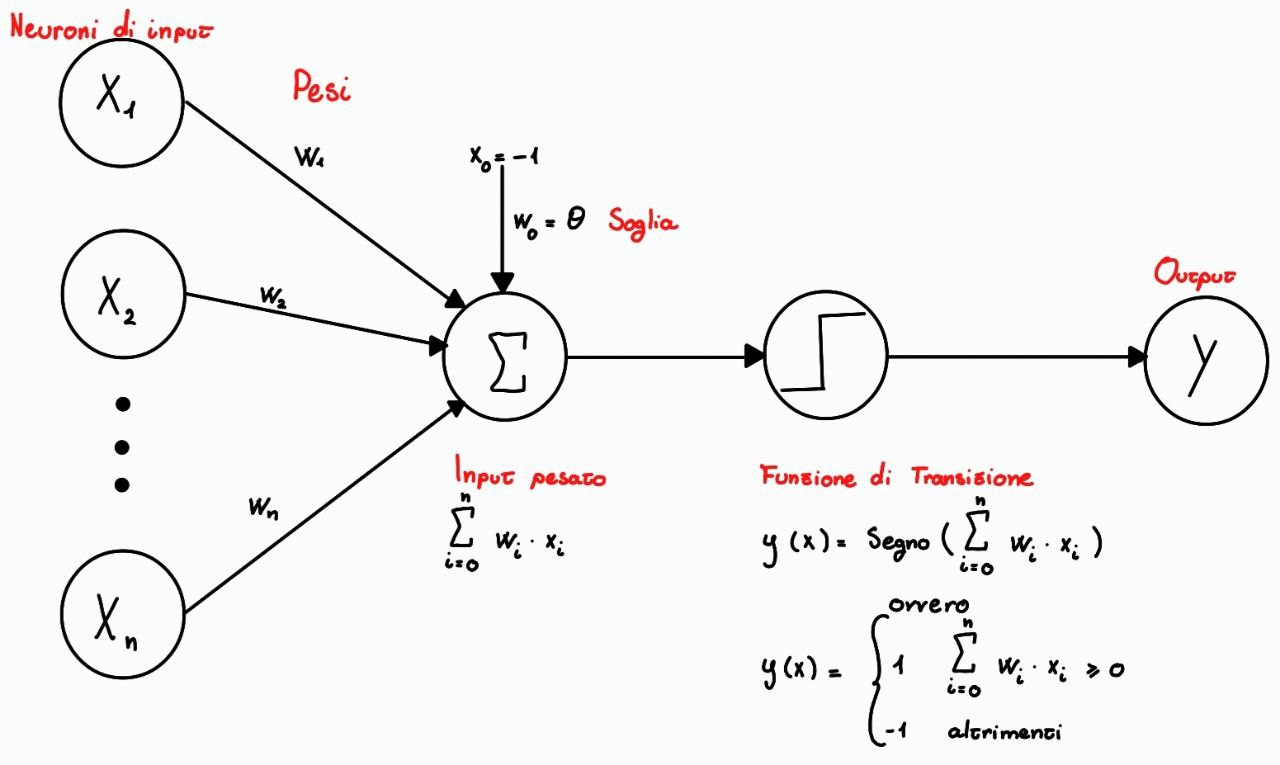
\includegraphics[width=0.7\textwidth]{img/reti/percettrone.png}
    \caption{Rappresentazione grafica del percettrone}
\end{figure}

Un percettrone è composto da un vettore di input $x_i$, ognuno con associato un
peso $w_i$. Oltre a questi, esso prende in input una soglia $\theta$, la quale è
trattata come il peso di una unità di input in stato fisso $x_0 = -1$. La transizione
di stato è determinata dal risultato del prodotto interno tra il vettore dei
pesi $\textbf{w}$ e il vettore degli stati di input $\textbf{x}$. Da un punto di
vista geometrico, il vettore dei pesi determina un iperpiano che separa i possibili
vettori di input in due classi, a seconda che formino con $\textbf{w}$ un angolo
acuto oppure ottuso.

Solitamente coi percettroni si parla di learning supervisionato.

Il processo di apprendimento di un percettrone parte assegnando in modo casuale
i pesi agli input. Questi pesi verranno modificati nella fase di apprendimento.

Se assumiamo che l'obiettivo è quello di separare i vettori in input in due classi
$A$ e $B$, possiamo utilizzare la seguente procedura per raggiungere questo scopo.
Si sottomette una sequenza infinita $\{x_k\}$ di vettori tale che ve ne siano un
numero infinito sia di $A$ che di $B$. Per ogni $x_k$ la rete calcola la risposta
$y_k$. Se la risposta è errata, si modificano i pesi nel seguente modo:
\begin{itemize}
    \item Incremento i pesi delle unità di input attive se si è risposto 0 anziché 1.
    \item Decremento i pesi delle unità di input attive se si è risposto 1 anziché 0.
\end{itemize}
\begin{equation}
    w' = w \pm x
\end{equation}

Vediamo due teoremi utili per lo studio dell'apprendimento del percettrone su due
classi $A$ e $B$, banalmente rappresentanti, nella nostra situazione binaria e
semplificata, il caso in cui si abbia il neurone che emette il segnale o altrimenti.
Nel nostro caso le classi sono discriminabili.
\begin{teorema}[\textbf{Teorema della convergenza}]
    Comunque si scelgano i pesi iniziali, se le classi $A$ e $B$ sono discriminabili,
    la procedura di apprendimento termina dopo un numero finito di passi.
\end{teorema}
\begin{teorema}[\textbf{Teorema di Minsky e Papert}]
    La classe delle forme discriminabili da un percettrone semplice è limitata
    alle forme linearmente separabili.
\end{teorema}

\begin{teorema}
    Se l'insieme degli input estesi è partito in due classi linearmente separabili
    $A$ e $B$ allora è possibile trovare un vettore di pesi $w$ tale che:
    \begin{equation}
        \begin{array}{ccc}
            \textbf{w} \cdot \textbf{x} \geq 0 & se & x \in A \\
            \textbf{w} \cdot \textbf{x} < 0    & se & x \in B
        \end{array}
    \end{equation}
\end{teorema}

Vediamo ora una nuova regola per aggiornare i pesi del percettrone:
\begin{equation}
    w'_i = w_i + \Delta w_i = w_i + \eta \cdot (t - y) \cdot x_i
\end{equation}
dove: \begin{itemize}
    \item $t$ rappresenta il valore del target.
    \item $y$ rappresenta l'output del percettrone.
    \item $\eta$ rappresenta il learning rate.
\end{itemize}

Così facendo si aggiornano i pesi del percettrone quando esso sbaglia la risposta.
Usando questa regola, l'algoritmo converge alla classificazione corretta se i
dati del training sono linearmente separabili e se $\eta$ assume un valore abbastanza piccolo.
\subsection{Discesa del gradiente}
Si consideri ora una unità lineare, con stati continui e un output calcolato come:
\begin{equation}
    y = w_0 + w_1x_1 + \dots + w_nx_x
\end{equation}
Una possibile strategia di apprendimento per questo modello consiste nel minimizzare
una opportuna funzione dei pesi $w_i$. Questo risultato può essere ottenuto cercando
di minimizzare l'errore ottenuto sul training set usando la discesa del gradiente:
\begin{equation}
    w' = w - \eta \cdot \nabla E[\textbf{w}]
\end{equation}
dove posso approssimare la discesa del gradiente come:
\begin{equation}
    \sum_d (t_d - y_d) (- x_i)
\end{equation}
Per effettuare questo aggiornamento abbiamo due modalità:
\begin{itemize}
    \item \textbf{Modalità Batch}: dove l'aggiornamento dei pesi viene calcolato
          rispetto all'intero insieme $D$.
          \begin{equation}
              w = w - \eta \cdot \nabla E_D[w] \ \text{con} \ E_D[w] = \frac{1}{2} \sum_{d \in D} (t_d - y_d)^2
          \end{equation}
          Esiste una variante chiamata \textbf{mini batch} che consiste nel dividere
          il dataset in $n$ porzioni e aggiornare i pesi ogni volta che si è
          analizzato un batch.
    \item \textbf{Modalità incrementale}: dove l'aggiornamento dei pesi viene
          calcolato rispetto a singoli esempi $d$.
          \begin{equation}
              w = w - \eta \cdot \nabla E_d[w] \ \text{con} \ E_d[w] = \frac{1}{2} (t_d - y_d)^2
          \end{equation}
          Questa modalità può approssimare la discesa del gradiente con la
          modalità Batch arbitrariamente se $\eta$ è abbastanza piccolo.
\end{itemize}

Rispetto a quanto visto per il percettrone la discesa lungo il gradiente converge
all'ipotesi con il minimo errore quadratico se $\eta$ è abbastanza basso, anche
per dati di training molto rumorosi.
\section{Reti neurali}
Fino ad ora abbia studiato il comportamento del singolo neurone, ma come per il
cervello umano, la forza di questo approccio è data dall'unione di più neuroni.
Per realizzare questo risultato la soluzione consiste nel collegare i neuroni in
modo da ottenere una struttura a grafo aciclico orientato. Così facendo, l'output
di un neurone diventa l'input di un altro.

Le reti neurali così composte hanno delle caratteristiche strutturali come:
\begin{itemize}
    \item hanno un gran numero di unità.
    \item permettono operazioni elementari.
    \item hanno un alto livello di interconnessione.
\end{itemize}
e delle caratteristiche dinamiche:
\begin{itemize}
    \item Si hanno cambiamenti di stato in funzione dello stato dei neuroni collegati
          in input.
    \item Si ha una funzione di uscita per ogni unità.
    \item Si ha la modifica dello schema di connessione, tramite la modifica dei
          pesi, per l'apprendimento.
\end{itemize}

L'output di un neurone è uno stato per un altro neurone. Si hanno alcuni elementi
caratterizzanti di una rete neurale:
\begin{itemize}
    \item Il tipo di unità.
    \item La topologia, ovvero la direzione delle connessioni, il numero di neuroni, $\dots$
    \item Le modalità di attivazione.
    \item Un algoritmo di apprendimento con lo studio dei pesi.
\end{itemize}

L'apprendimento di un neurone modifica i pesi sinaptici. Se due neuroni connessi
sono per più volte di seguito contemporaneamente attivi, il peso della sinapsi aumenta.
\begin{figure}[!ht]
    \centering
    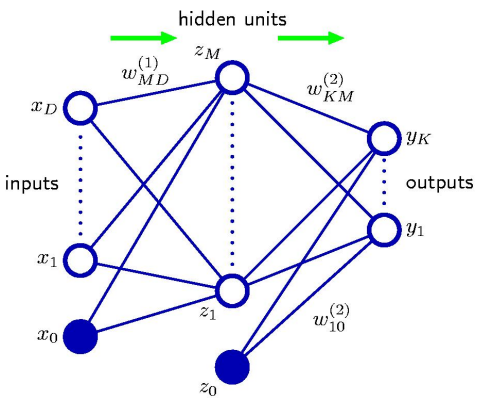
\includegraphics[width=0.6\textwidth]{img/reti/rete.png}
    \caption{Rete Neurale multi strato}
\end{figure}

Dal punto di vista formale, dovendo espandere le definizioni fatte nel caso del
singolo neurone a più neuroni, si lavora con:
\begin{itemize}
    \item $D$ le variabili di input $x_1, \dots, x_D$.
    \item Una matrice dei pesi $W$, con i valori indicati tramite $w_{ij}$, per
          gli archi che collegano i neuroni. I pesi sono i pesi correnti.
    \item Un vettore delle soglie $\Theta$, con i valori indicati tramite $\theta_i$,
          una per ogni neurone.
    \item L'input netto per il neurone $i$ al tempo $t$, indicato con:
          \begin{equation}
              n_i(t) = \sum_{j = 1}^n w_{ij} \cdot x_j(t) - \theta_i
          \end{equation}
          quindi si ha che la soglia influisce già nell'input del neurone e quindi
          $\theta_i$ viene considerata come soglia di azzeramento del valore entrante.
    \item La funzione di transizione indicata con:
          \begin{equation}
              s_i(t + 1) = g(n_i(t))
          \end{equation}
    \item $M$ ovvero il numero delle unità di attivazione nascoste:
          \begin{equation}
              a_j = \sum_{i = 1}^D w_{ji}^{(1)}x_i + w_{j0}^{(1)}
          \end{equation}
          dove $j = 1, \dots, M$.
    \item $z_j = h(a_j)$ come le funzioni di attivazione nascoste.
    \item $K$ ovvero il numero delle unità di attivazione in output:
          \begin{equation}
              a_k = \sum_{i = 1}^M w_{ki}^{(2)}x_i + w_{k0}^{(2)}
          \end{equation}
          dove $k = 1, \dots, K$.
    \item Indichiamo con $y_k = \sigma(a_k)$ la funzione di attivazione dell'ultimo strato.
          \begin{equation}
              y_k(\textbf{x}, \textbf{w}) = \sigma \left(\sum_{j = 1}^M w_{kj}^{(2)} \cdot h \left(\sum_{i = 1}^D w_{ji}^{(1)}x_i + w_{j0}^{(1)}\right) + w_{k0}^{(2)}\right)
          \end{equation}
\end{itemize}

I singoli \textit{percettroni} ci permettono di costruire delle frontiere di
separazione lineari, questo però limita l'applicabilità di questa tecnica. Nel
caso in cui si ha la volontà di costruire frontiere di separazione non lineari è
necessario combinare più neuroni $u_i$, anche posizionati in strati intermedi tra
input e output, andando a formare una rete.

Per questa modifica si passa dalla funzione di attivazione a gradino a una funzione
di attivazione derivabile, ovvero la sigmoide:
\begin{equation}
    \sigma(x) = \frac{1}{1 + e^{-x}}
\end{equation}
Questa scelta viene fatta per semplificare la fase di aggiornamento dei pesi.

A questo punto, per ogni configurazione in ingresso al primo strato $x$, la rete
calcola una configurazione $y$ dell'ultimo strato.

L'obiettivo è fissata una mappa $f$ tra configurazioni di ingresso e di uscita,
sulla base di una sequenza di stimoli $x_k$, la rete cambia i pesi $w_{ij}$ in
modo che, dopo un numero finito $s$ di passi l'uscita $y_k$ coincida con $f(x_k)$
per ogni $k > s$, almeno approssimativamente. Il criterio di apprendimento della
rete consiste nel minimizzare la discrepanza tra il target atteso e la previsione della rete.

Nella fase di addestramento l'obiettivo è quello di determinare i pesi $w$ da
assegnare alle connessioni della rete partendo da un training set. La procedura di
apprendimento è composta da due step:
\begin{enumerate}
    \item Valutare il gradiente dell'errore $\nabla E(w)$ rispetto ai pesi $w_1, \dots, w_T$.
    \item Usare il vettore di derivate ottenuto per calcolare i nuovi pesi.
\end{enumerate}
\begin{equation}
    w^{(\tau + 1)} = w^{(\tau)} - \eta \cdot \nabla E(w^{(\tau)})
\end{equation}

Usando un \textbf{Computational Graph} possiamo rappresentare una funzione composta
come un grafo aciclico orientato dove ogni nodo rappresenta una funzione o un
operazione e ogni arco rappresenta l'input per il nodo.

Possiamo calcolare la derivata di una funzione composta $f(g(h(x)))$ come:
\begin{equation}
    \frac{df}{dx} = \frac{df}{dg} \cdot \frac{dg}{dh} \cdot \frac{dh}{dx}
\end{equation}
\subsection{Backpropagation}
Quando si lavora con le reti l'aggiornamento dei pesi risulta più complicato
rispetto a quando si lavora con il singolo neurone. Infatti, nel caso delle reti
l'errore lo sappiamo solamente alla fine. Risulta quindi difficile il processo di
aggiornare gli stati intermedi.

Quando si lavora con più strati, l'aggiornamento dei pesi viene ottenuto per mezzo
di una derivata della funzione composta.

Abbiamo quindi l'algoritmo di \textbf{Backpropagation} che si divide in 5 passi:
\begin{enumerate}
    \item \textbf{Input}: al neurone di input $u_j$ viene assegnato lo stato $x_j$.
    \item \textbf{Propagazione}: si calcola lo stato dei neuroni nascosti o di output $u_j$:
          \begin{equation}
              s_j = f_j(n_j)
          \end{equation}
          dove $n_j$ è l'input netto al neurone $u_j$ e si calcola come:
          \begin{equation}
              n_j = \sum_{i = 0}^n w_{ij} \cdot s_i
          \end{equation}
    \item \textbf{Confronto}: per ogni neurone di output $u_j$, noto l'output
          atteso $t_j$, si calcola:
          \begin{equation}
              \delta_j = f'_j(n_j) \cdot (t_j - y_j)
          \end{equation}
          Possiamo vedere la propagazione in avanti nella rete si ottiene come
          moltiplicazione tra matrici. In particolare, ogni strato è in funzione
          dello strato precedente.
    \item \textbf{Retropropagazione dell'errore}: per ogni neurone nascosto $u_j$,
          si calcola:
          \begin{equation}
              \delta_j = f_j'(n_j) \cdot \left( \sum_{h} w_{jh} \cdot \delta_h \right)
          \end{equation}
    \item \textbf{Aggiornamento dei pesi}: si ha:
          \begin{equation}
              w_{ij} = w_{ij} + \eta \cdot \delta_i \cdot s_j
          \end{equation}
\end{enumerate}

Vediamo quindi una possibile implementazione dell'algoritmo:
\begin{algorithm}[H]
    \begin{algorithmic}
        \Function{Backpropagation}{}
        \State \textit{inizializzo ogni $\Delta w_i$ ad un valore piccolo casuale}
        \While {\textit{non raggiungimento della condizione di terminazione}}
        \For {\textit{ogni esempio $\langle (x_1,\ldots, x_n),t\rangle$}}
        \State \textit{immetto l'input $( x_1, \ldots x_n)$ nella rete e calcolo
            $y_k$}
        \For {\textit{ogni unità di output $k$}}
        \[\delta_k=y_k\cdot(1-y_k)\cdot(t_k-y_k)\]
        \EndFor
        \For {\textit{ogni unità nascosta $h$}}
        \[\delta_h=y_h\cdot(1-y_h)\cdot\sum_k w_{hk}\delta_k\]
        \EndFor
        \For {\textit{ogni peso $w_{ij}$}}
        \[w_{ij}=w_{ij}+\Delta w_{ij},\mbox{ con } \Delta w_{ij}=\eta\cdot\delta_j\cdot x_{ij}\]
        \EndFor
        \EndFor
        \EndWhile
        \State \textit{aggiorno i pesi:}
        \[w_i=w_i+\Delta w_i\]
        \EndFunction
    \end{algorithmic}
    \caption{Algoritmo di Backpropagation}
\end{algorithm}

Si trova però un minimo locale e non globale e spesso include termini di \textit{momento}
per cambiare la formula dell'aggiornamento dei pesi del tipo:
\begin{equation}
    \delta w_{ij}(n) = \eta \cdot \delta_j \cdot x_{ij} + \alpha \cdot \Delta w_{ij} (n - 1)
\end{equation}
in modo da avere una sorta di inerzia per la variazione dei pesi. Esistono
tecniche che permettono di "uscire" dai minimi locali.

Si minimizzano gli errori sugli esempi di training ma si rischia l'overfitting.

Tutti questi fattori comportano un addestramento lento, ma dopo l'addestramento
si ha una rete veloce.
\subsection{Overfitting}
Più la rete è ricca di neuroni e pesi e più può imparare semplicemente "fotografando"
nella sua memoria le istanze, questo porta a una situazione di overfitting.

Un idea per limitarlo consiste nel penalizzare la rete durante il training, ovvero
costringo la rete a generalizzare cogliendo regolarità nelle istanze, invece di
"fotografarle". In generale queste sono dette tecniche di \textbf{regolarizzione}.

Esistono diverse tecniche per limitare l'overfitting, una di queste è chiamata
\textbf{dropout}. Questa tecnica consiste nello spegnere un determinato numero di
neuroni in modo da obbligare la rete a generalizzare.
\subsection{Utilizzi}
Uno degli utilizzi delle reti neurali è quello di ridurre la dimensionalità dei
dati mantenendo le informazioni essenziali. Questo risultato può essere ottenuto
anche con tecniche che non richiedono l'uso di reti neurali, ad esempio utilizzando
una tecnica nota come \textbf{PCA} (\textit{Principal Component Analysis}). L'idea
dietro questa tecnica consiste nel trovare una trasformazione lineare delle
caratteristiche che massimizza la varianza o minimizza l'errore quadratico di
ricostruzione.

Gli \textbf{Autoencoder} sono delle reti neurali che mi permettono di codificare
gli input utilizzando poche informazioni. Questo particolare modello di rete neurale
è unsupervised e viene addestrata in modo che l'input sia uguale all'output. Per
riuscire a ridurre la codifica dell'input la rete è composta da due parti che sono
collegate tra di loro una dopo l'altra:
\begin{itemize}
    \item \textbf{Encoder}: si occupa di prendere l'input e ridurlo di dimensionalità.
    \item \textbf{Decoder}: partendo dalla codifica in pochi bit ricostruisce l'input originale.
\end{itemize}
\begin{figure}[!ht]
    \centering
    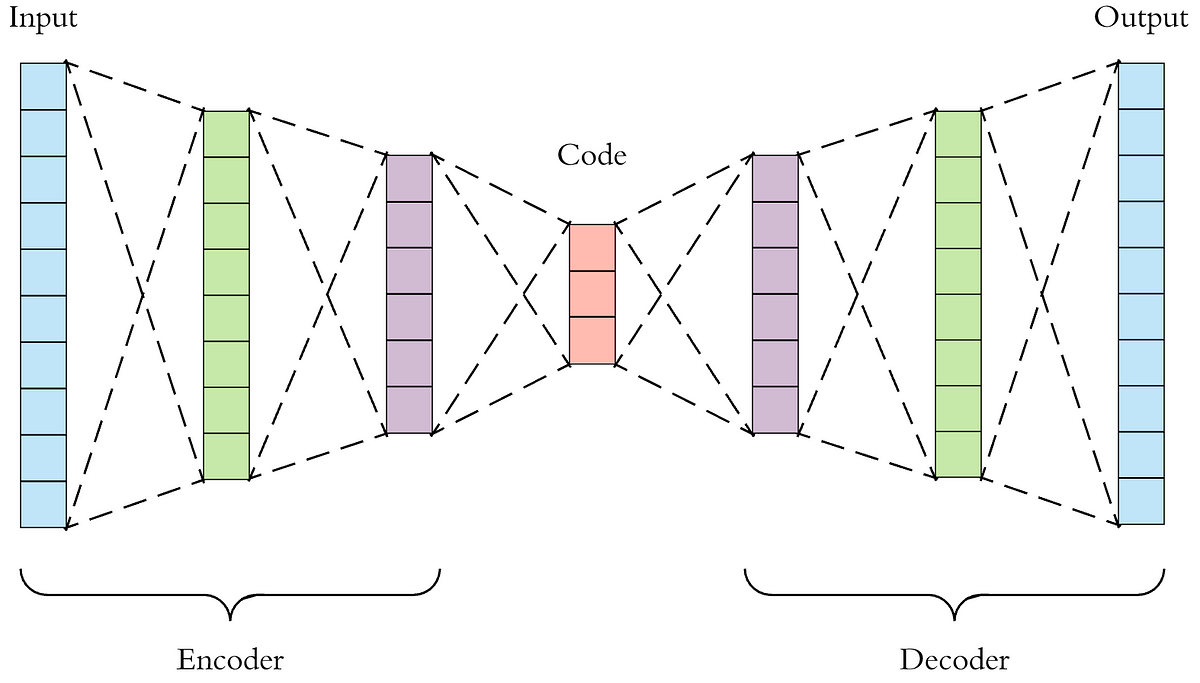
\includegraphics[width = 0.6\textwidth]{img/reti/autoencoder.png}
    \caption{Struttura di un Autoencoder}
\end{figure}

Oltre a questo si cerca di trasformare features categoriche in features numeriche
in modo da semplificare i processi di apprendimento.
\subsection{Limiti}
Si hanno quindi i seguenti limiti:
\begin{itemize}
    \item Mancanza di teoremi generali di convergenza.
    \item Può portare in minimi locali di E.
    \item Difficoltà per la scelta dei parametri.
    \item Scarsa capacità di generalizzazione.
\end{itemize}
Si possono però avere varianti che permettono di migliorare il modello tramite:
\begin{itemize}
    \item Un tasso di apprendimento adattivo: $\eta = g(\nabla E)$
    \item Range degli stati da $-1$ a $1$.
    \item L'uso di termini di momento.
    \item Deviazioni dalla discesa più ripida.
    \item Variazioni nell'architettura (numero di strati nascosti)
    \item Inserimento di connessioni all'indietro.
\end{itemize}

\begin{osservazione}
    Rispetto alberi decisionali si ha:
    \begin{itemize}
        \item Le reti neurali sono più lente in fase di apprendimento ma uguali
              in fase di esecuzione.
        \item Le reti neurali hanno una migliore tolleranza del rumore.
        \item Le reti neurali risultano più complesse da capire.
    \end{itemize}

    Si nota che ne le reti neurali ne gli alberi decisionali possono usare della
    conoscenza a priori.
\end{osservazione}
\chapter{Support Vector Machines}
Precedentemente abbiamo introdotto:
\begin{itemize}
    \item \textbf{Percettrone semplice}: è un algoritmo di apprendimento efficiente
          solo per funzioni di separazione lineare.
    \item \textbf{Percettrone multistrato}: è un algoritmo difficile da addestrare
          perché deve aggiornare molti pesi e ci sono molti minimi locali, apprende
          sia funzionil lineari che non lineari.
\end{itemize}
Le \textbf{Support Vector Machines} (SVM) sono un algoritmo efficiente per
apprendere funzioni di separazione non lineari complesse.

Anche nel caso delle SVM viene ripreso comunque il concetto di separazione lineare
ma con una scelta dell'iperpiano migliore. Si usa la \textit{teoria statistica
    dell'apprendimento}, utilizzando la \textbf{programmazione matematica}, la quale
dice che tra tutti gli iperpiani che possiamo usare per separare due classi, si
sceglie quello che sia in grado di etichettare meglio nel futuro. L'intuizione
è quella di prendere un iperpiano ottimo rispetto alla misura della distanza minima
che si ha tra gli esempi. Si guardano quindi tutti i punti del training set e
cerco di piazzare in mezzo l'iperpiano, in modo che intorno ad esso ci sia massima
ampiezza. Tale ampiezza è detta \textbf{margine}.
\begin{definizione}[\textbf{Margine}]
    Il margine è la distanza tra i vettori di supporto e l'iperpiano.
\end{definizione}
Se riuscissimo a separare i dati con un largo margine avremmo ragione di credere
che il classificatore sia “più robusto” tanto da avere una migliore generalizzazione.
Quando arriva quindi un nuovo punto, generato con la stessa regola degli altri,
\textit{sarà sicuramente} classificato correttamente, una volta scelto l'iperpiano.

Ci serve quindi la separabilità delle istanze, serve quindi che la funzione generatrice
sia linearmente separabile.
\begin{teorema}[\textbf{Dimensione di Vapnik-Cervonenkis}]
    Con la teoria statistica dell'apprendimento si dimostra che più allarghiamo
    il margine meglio l'iperpiano generalizza, raggiungendo la dimensione di
    Vapnik-Cervonenkis (VC). Prese tutte le funzioni che generano il training
    set si produce la Vapnik-Cervonenkis che esprime quanto è difficile sbagliare
    sulle ipotesi future in base alla scelta dell'iperpiano.
\end{teorema}
Dobbiamo quindi scrivere un algoritmo per trovare l'iperpiano di separazione di
massimo margine. In input si hanno le istanze etichettate e in output un vettore
che identifica l'iperpiano. Viene usata una notazione matematica, la quale prevede
che, preso un insieme di punti di training:
\begin{equation}
    S = \{(x_1, y_1), (x_2, y_2),\dots, (x_n, y_n)\}
\end{equation}
dove ad ogni vettore $x_i$ associo la classe di appartenenza $y_i$:
\begin{equation}
    y_i \in \{-1, +1\}
\end{equation}
ho i punti linearmente separabili nel seguente modo:
\begin{equation}
    \begin{cases}
        \langle w, x_i \rangle + b > 0 & \text{se} \ y_i = +1 \\
        \langle w, x_i \rangle + b < 0 & \text{se} \ y_i = -1
    \end{cases}
\end{equation}
questo può essere riassunto in un solo vincolo nel seguente modo:
\begin{equation}
    y_i(\langle w, x_i\rangle + b) > 0, \  i = 1,\dots, n
\end{equation}
Si ha che il vettore $w$ mi dirà l'inclinazione del piano mentre $b$ è la distanza
tra l'origine e il piano, queste due variabili identificano i vari iperpiani
possibili tra cui cercare il migliore.

L'ipotesi quindi tra $w$ e $b$ è una funzione che prende il segno di $\langle w,
    x \rangle + b$ per associare l'etichetta:
\begin{equation}
    h_{w,b} (x) = sgn(\langle w, x \rangle + b)
\end{equation}
Siano $d_{-}$ e $d_{+}$ le distanze tra l'iperpiano separatore e il punto positivo
e negativo più vicino, allora definiamo:
\begin{itemize}
    \item \textbf{Margine funzionale}.
    \item \textbf{Margine geometrico}.
\end{itemize}
\begin{definizione}[\textbf{Margine funzionale}]
    Definiamo il \textbf{margine funzionale} di un punto $(x_i, y_i)$ rispetto
    all'iperpiano $(w, b)$ come:
    \begin{equation}
        \hat{\gamma}_i = y_i( \langle w, x_i \rangle + b )
    \end{equation}
    e quindi il margine funzionale dell'iperpiano rispetto al training set $S$ è
    definito come:
    \begin{equation}
        \hat{\rho} = \min_{i = 1, \dots, n} \hat{\gamma}_i
    \end{equation}
\end{definizione}
Si hanno quindi due casistiche:
\begin{enumerate}
    \item Se si ha un punto $x_i$ tale che $y_i = +1$, perché il margine
          funzionale sia grande è necessario che la quantità $\langle w, x_i
              \rangle + b$ abbia un grande valore positivo.
    \item Se si ha un punto $x_i$ tale che $y_i = -1$, perché il margine funzionale
          sia grande è necessario che la quantità $\langle w, x_i \rangle + b$
          abbia un grande valore negativo.
\end{enumerate}
Il margine funzionale specifica quanta è buona la classificazione, ma non misura
la distanza degli esempi dall'iperpiano.
\begin{teorema}
    Se $\hat{\gamma}_i > 0$, per ogni $classificazione_i$ la classificazione è
    approvata in quanto le classi sono linearmente separabili e l'iperpiano
    $(w, b)$ separa effettivamente le classi
\end{teorema}
Si ha quindi che un ampio margine funzionale fornisce una maggior qualità
di previsione, anche, se l'uso del solo $\hat{\gamma}$ può essere problematico,
in quanto il margine funzionale non è invariante rispetto ad un iperpiano ri-scalato.

Per come è stato scelto il classificatore $f$, se si scala l'iperpiano:
\begin{equation}
    (w, b) \to (c \cdot w, c\cdot b)
\end{equation}
si ottengono:
\begin{itemize}
    \item Lo stesso iperpiano, ovvero lo stesso luogo di punti.
    \item La stessa funzione di decisione, visto che quest'ultima dipende solo
          dal segno di $\langle w, x \rangle + b$, con il segno che può essere
          invertito se $c < 0$.
\end{itemize}
ma dato che il margine funzionale viene moltiplicato per $c$, non possiamo usarlo
come distanza di un punto dall'iperpiano, perché non è \textbf{invariante} rispetto
alla scala. Bisogna studiare la distanza $d$ del punto $x$ dall'iperpiano. Si ha
quindi:
\begin{equation}
    d = \frac{\sum_{i = 1} ^ n w_i \cdot x_i + b}{\| w \|} =
    \frac{\langle w, x_i \rangle + b}{\|  w \|}
\end{equation}
\begin{definizione}[\textbf{Margine geometrico}]
    Definiamo il \textbf{margine geometrico} di un punto $(x_i, y_i)$ rispetto
    all'iperpiano $(w, b)$ come:
    \begin{equation}
        \gamma = \frac{y_i(\langle w, x_i \rangle + b)}{\| w \|}
    \end{equation}
    e quindi il margine geometrico dell'iperpiano rispetto al training set $S$ è
    definito come:
    \begin{equation}
        \rho =  \min_{i = 1, \dots, n} {\gamma}_i
    \end{equation}
\end{definizione}
A differenza del margine funzionale, il margine geometrico ci specifica quanto
sono distanti i punti dall'iperpiano.
\begin{teorema}
    Se $\gamma_i > 0$, per ogni $classificazione_i$ la classificazione è approvata
    analogamente a quanto detto per il margine funzionale.
\end{teorema}
Dato un punto positivo/negativo il margine geometrico rappresenta la sua distanza
geometrica dall'iperpiano, il margine geometrico rende meglio l'idea della distanza
di un punto da un iperpiano in $\mathbb{R}^n$.

Inoltre, si ha che il margine geometrico è invariante rispetto alla scala di $w$
e quindi possiamo scalare l'iperpiano senza cambiamenti della distanza dei punti
rispetto all'iperpiano, in questo modo il margine rimane invariato. Al contrario
il margine funzionale è variante perché cambiando la scala di $w$ allora cambiava
anche il valore del margine, cambiando la semantica della classificazione, ciò
comporta errori.

Dalla formula notiamo che, posto $\| w \| = 1$ si scala l'iperpiano $(w, b)$:
\begin{equation}
    (w, b) \to \left(\frac{w}{\|w\|}, \frac{b}{\| w\|}\right)
\end{equation}
Si considera quindi un iperpiano $\left(\frac{w}{\|w\|}, \frac{b}{\| w\|}\right)$
con il vettore di pesi $\frac{w}{\| w \|}$ di norma unitaria.
\begin{definizione}[\textbf{Iperpiano canonico}]
    Definiamo un \textbf{iperpiano canonico} se:
    \begin{equation}
        \min_{i = 1, \dots, n} |\langle w, x_i \rangle + b| =  1
    \end{equation}
    e quindi, per un iperpiano canonico si hanno:
    \begin{itemize}
        \item margine funzionale pari a $1$
        \item margine geometrico pari a $\frac{1}{\| w \|}$
    \end{itemize}
\end{definizione}
Si nota che se $\| w \| = 1$ allora margine funzionale e geometrico coincidono,
infatti si possono mettere in correlazione:
\begin{equation}
    \gamma = \frac{\hat{\gamma}}{\| w \|}
\end{equation}
Bisogna quindi cercare di estendere il margine, cerchiamo quindi di massimizzare
una certa funzione obiettivo:
\begin{equation*}
    \begin{aligned}
        \max f(x) \\ \text{s.t.} \ g(x) \leq 0 \\ h(x) = 0
    \end{aligned}
\end{equation*}
Vorremmo assicurarci che tutti i punti cadano al di fuori del margine e quindi,
dato un certo $\gamma$ vogliamo, $\forall i \in \{1, \dots, n\}$:
\begin{equation}
    \frac{y_i \cdot (\langle w, x_i \rangle + b)}{\| w \|} \geq \gamma
\end{equation}
e quindi vogliamo:
\begin{equation*}
    \begin{aligned}
        \max \gamma \\ \text{s.t.} \ y_i (\langle w, x_i \rangle + b) \leq
        \gamma      \\ \| w \| = 1
    \end{aligned}
\end{equation*}
avendo, con il secondo vincolo, margine geometrico uguale a quello funzionale.
Riscriviamo quindi:
\begin{equation*}
    \begin{aligned}
        \max \frac{\hat{\gamma}}{\|w\|} \\ \text{s.t.} \ y_i(\langle w, x_i
        \rangle + b) \leq \gamma
    \end{aligned}
\end{equation*}
Non avendo comunque un vincolo convesso.

Possiamo però scalare l'iperpiano senza variazioni, grazie all'invarianza.
Lo scalo quindi in modo da avere l'iperpiano canonico, con margine funzionale
pari a 1:
\begin{equation*}
    \begin{aligned}
        \max \frac{1}{\|w\|} \\ \text{s.t.} \ y_i(\langle w, x_i \rangle + b)
        \leq \gamma
    \end{aligned}
\end{equation*}
Si cerca quindi di rendere massimo $\frac{1}{\|w\|}$ che equivale a rendere
minimo $\frac{1}{2} \| w \|^2$. Quindi si ottiene che vogliamo minimizzare
$\frac{1}{2} \| w \|^2$, che per comodità chiamiamo $\tau (w)$:
\begin{equation*}
    \begin{aligned}
        \max \tau(w) = \frac{1}{2}  \| w\|^2 \\ \text{s.t.} \ y_i (\langle w, x_i
        \rangle + b) \leq \gamma
    \end{aligned}
\end{equation*}
\begin{teorema}
    Si dimostra che esiste una sola soluzione al problema, ovvero esiste un unico
    iperpiano di massimo margine.
\end{teorema}
Ricapitolando si hanno due ragioni a supporto delle SVM:
\begin{enumerate}
    \item La generalizzazione, ovvero la capacità dell'iperpiano di separazione
          di massimo margine.
    \item Esiste un'unica soluzione del problema di ottimizzazione appena descritto.
\end{enumerate}
Si sta cercando:
\begin{equation*}
    \begin{aligned}
        \max \tau(w) = \frac{1}{2}  \| w\|^2 \\ \text{s.t.} \ y_i (\langle w, x_i
        \rangle + b) \leq \gamma
    \end{aligned}
\end{equation*}
e si ha che:
\begin{equation}
    w = \sum_{i \in Q} \alpha_i \cdot x_i
\end{equation}
ovvero scritta in termini di un sottoinsieme di esempi del training set che
giacciono sul margine dell'iperpiano, anche noto come \textbf{vettori di supporto},
prendendo una somma pesata dei contenuti dei vettori.

Il passaggio finale è che, se ho $\langle w, x \rangle + b$ che indicano cosa ho
appreso, se ricevo un vettore $x$ da classificare posso determinare l'etichetta:
\begin{equation}
    sgn(\langle w, x \rangle + b) = sgn\left(\left\langle \sum_{i \in Q} \alpha_i
    \cdot x_i, x \right\rangle + b \right) = sgn\left(\sum_{i \in Q} \alpha_i
    \cdot \langle x_i, x\rangle + b \right)
\end{equation}
Quindi la funzione di decisione associata alla soluzione può essere scritta in
termini del prodotto interno tra i vettori di supporto (support vector) $x_i$ e
il vettore da classificare $x$.
\section{Punti non sono linearmente separabili}
Quando si lavora con punti non lineare separabili si usa lo stesso approccio,
rivedendo la formulazione del problema tramite i \textbf{metodi kernel}.
Si cerca di mappare lo spazio di input in un nuovo spazio che è a dimensione maggiore
in cui i punti siano linearmente separabili, in questo modo è possibile classificare
anche esempi non separabili linearmente.

Per effettuare questa trasformazione, dobbiamo trovare una funzione che prende
il nome di \textbf{funzione di trasformazione}:
\begin{equation}
    \Phi: \mathbb{R}^n \to \mathbb{R}^m, \ \text{con} \ m > n
\end{equation}
che mappi i dati iniziali non linearmente separabili in uno spazio di dimensione
superiore in cui siano linearmente separabili.

In questo nuovo spazio la funzione di decisione che classifica l'input $x$ è:
\begin{equation}
    sgn\left(\sum_{i \in Q} \alpha_i \cdot \langle \Phi(x_i), \Phi(x)\rangle + b
    \right)
\end{equation}
Il calcolo delle funzioni di trasformazione $\Phi$ è generalmente computazionalmente
pesante ma è semplificato nel caso di funzioni kernel.
\begin{definizione}[\textbf{Funzione kernel}]
    Data una trasformazione $\Phi: \mathbb{R}^n \to \mathbb{R}^m$ una
    \textbf{funzione kernel} è una mappa:
    \begin{equation}
        K: \mathbb{R}^n \times \mathbb{R}^n \to \mathbb{R} \ \text{tale che} \
        K(x, y) = \Phi(x) \cdot \Phi(y)
    \end{equation}
\end{definizione}
\begin{definizione}[\textbf{Kernel trick}]
    Si definisce quindi il \textbf{kernel trick} ovvero una procedura che permette
    di computare il prodotto interno delle trasformazioni dei due vettori $x$ e
    $y$, ovvero $\langle\Phi(x), \ \Phi(y)\rangle$, senza computare le
    trasformazioni. Questo permette di semplificare il calcolo di:
    \begin{equation}
        sgn\left(\sum_{i \in Q} \alpha_i \cdot \langle \Phi(x_i), \Phi(x) \rangle
        + b \right)
    \end{equation}
    sostituendo $\langle\Phi(x), \ \Phi(y)\rangle$ con $K(x_i, x)$, ottenendo:
    \begin{equation}
        sgn\left(\sum_{i \in Q} \alpha_i \cdot K(x_i, x) + b \right)
    \end{equation}
\end{definizione}
\begin{nota}
    Non si cercano tutte le possibili trasformazioni ma solo alcune.
\end{nota}
\begin{esempio}
    Sia $\Phi:\mathbb{R}^2\rightarrow\mathbb{R}^3$ la funzione di trasformazione
    definita nel seguente modo:
    \begin{equation}
        \Phi(x,y) =(x^2,y^2,\sqrt{2xy})
    \end{equation}
    avremo che $p_1 = (x_1, y_1), p_2 = (x_2, y_2) \in \mathbb{R}^2$, allora ho
    $K(p_1, p_2) = \langle \Phi(p_1), \Phi(p_2) \rangle \in\mathbb{R}^3$,
    più precisamente:
    $$K(p_1,p_2) = \left\langle\left(\begin{array}{c}
                x_1^2 \\
                y_1^2 \\
                \sqrt{2x_1y_1}
            \end{array}\right),\left(\begin{array}{c}
                x_2^2 \\
                y_2^2 \\
                \sqrt{2x_2y_2}
            \end{array}\right)\right\rangle = (x_1 \cdot x_2)^2 + (y_1 \cdot
        y_2)^2 + 2 \sqrt{x_1 \cdot y_1 \cdot x_2 \cdot y_2}$$
\end{esempio}
Si hanno alcune proprietà:
\begin{itemize}
    \item Se i dati sono mappati in uno spazio di dimensioni sufficientemente
          elevate, saranno quasi sempre linearmente separabili.
    \item Quattro dimensioni sono sufficienti per separare linearmente un cerchio
          in qualsiasi punto del piano.
    \item Cinque dimensioni sono sufficienti per separare linearmente qualsiasi
          ellisse.
    \item Se abbiamo $N$ esempi sono sempre separabili in spazi di dimensioni
          $N - 1$ o più.
    \item Calcolare $K(x, y)$ può essere molto economico anche se $\Phi(x)$ è
          molto costoso, ad esempio con vettori di dimensione elevata e, in tali
          casi (che vanno dimostrati), si addestrano le SVM nello spazio di
          dimensionalità maggiore senza mai dover trovare o rappresentare
          esplicitamente i vettori $\Phi(x)$.
\end{itemize}
Vediamo una lista di kernel standard:
\begin{itemize}
    \item \textbf{Lineare}: $K(x, y) = x \cdot y$
    \item \textbf{Polinomiale}: $K(x, y) = (1 + x \cdot y)^d$
    \item \textbf{Radial basis function}: $K(x, y) = e^{-\gamma \| x - y\|^2}$
    \item \textbf{Gaussian radial basis function}: $K(x, y) = e^{\frac{-(x-y)^2}
                      {2 \cdot \sigma^2}}$
    \item \textbf{Percettrone multistrato}: $K(x, y) = \tanh(b(x \cdot y) - c)$
\end{itemize}
\begin{teorema}
    Un kernel definisce una matrice $K_{i,j}$ che è simmetrica e definita positiva.
\end{teorema}
\begin{teorema}[\textbf{Teorema di Mercer}]
    Ogni matrice simmetrica e definita positiva è un kernel.
\end{teorema}
\begin{definizione}[\textbf{Gram matrix}]
    Definiamo \textbf{kernel matrix}, detta anche \textbf{matrice di Gram},
    dato un kernel $K$ e un insieme di punti $x_1, \dots, x_n$ come una matrice
    dove ogni componente è:
    \begin{equation}
        G_{i, j} = \langle \Phi(x_i), \Phi(x_j) \rangle = K(x_i, x_j)
    \end{equation}
\end{definizione}
\begin{esempio}
    Considerando il seguente dataset:
    \begin{equation}
        x_1 = [1, 2], \ x_2 = [3, 4], \ x_3 = [5, 6]
    \end{equation}
    dove a ogni istanza è associata la rispettiva classe:
    \begin{equation}
        y_1 = 1, \ y_2 = -1, \ y_3 = 1
    \end{equation}
    e il seguente kernel:
    \begin{equation}
        K(x, y) = x^T \cdot y
    \end{equation}
    si vuole calcolare la matrice di Gram per il kernel $K$ usando il dataset.
    Dalla definizione della matrice di Gram si ha che:
    \begin{equation}
        G = \left[
            \begin{array}{ccc}
                K(x_1, x_1) & K(x_1, x_2) & K(x_1, x_3) \\
                K(x_2, x_1) & K(x_2, x_2) & K(x_2, x_3) \\
                K(x_3, x_1) & K(x_3, x_2) & K(x_3, x_3) \\
            \end{array}
            \right] = \left[
            \begin{array}{ccc}
                1 \cdot 1 + 2 \cdot 2 & 1 \cdot 3 + 2 \cdot 4 & 1 \cdot 5 + 2 \cdot 6 \\
                3 \cdot 1 + 4 \cdot 2 & 3 \cdot 3 + 4 \cdot 4 & 3 \cdot 5 + 4 \cdot 6 \\
                5 \cdot 1 + 6 \cdot 2 & 5 \cdot 3 + 6 \cdot 4 & 5 \cdot 5 + 6 \cdot 6 \\
            \end{array}
            \right] = \left[
            \begin{array}{ccc}
                5  & 11 & 17 \\
                11 & 25 & 39 \\
                17 & 39 & 61 \\
            \end{array}
            \right]
    \end{equation}
\end{esempio}
\section{Classificazione multi-classe}
SVM può essere applicato a problemi non binari tramite \textit{one vs rest},
ovvero consiste nell'effettuare, per ogni classe, un'esecuzione di SVM tra la singola classe
contro tutte le altre. In aggiunta, si combinano tutti gli iperpiani trovati
tra di loro per effettuare la classificazione multi-classe.

Si ha quindi l'addestramento di un singolo classificatore per classe, con i campioni
di quella classe considerati come positivi e tutti gli altri campioni come negativi.

Questa strategia richiede che i classificatori di base producano un punteggio di
confidenza a valore reale per la sua decisione, piuttosto che solo un'etichetta
di classe; infatti, le sole etichette di classi discrete possono portare a ambiguità.
Abbiamo quindi:
\begin{itemize}
    \item Come input:
          \begin{itemize}
              \item Un learner $L$
              \item Un set di esempi $X$
              \item Delle label $y_i$ associate ad ogni $x_i \in X$ con $i = 1, \dots, K$
          \end{itemize}
    \item Come output una lista di classificatori $f_k$ con $l = 1,\dots, K$
\end{itemize}
La procedura è quindi, $\forall k \in \{1 \dots K\}$ costruisco un nuovo vettore
di label $z$ tale che:
\begin{equation}
    \begin{cases}
        z_i = y_i & \text{se} \ y_i = k \\
        z_i = 0   & \text{altrimenti}
    \end{cases}
\end{equation}
applicando poi $L$ a $(x, z)$ per ottenere $f_k$.

Quindi prendere decisioni significa applicare tutti i classificatori ad un nuovo
esempio e prevedere l'etichetta $k$ per la quale il classificatore corrispondente
riporta il punteggio di confidenza più alto:
\begin{equation}
    \hat{y} = argmax f_k(x), \ k \in \{1,\dots K\}
\end{equation}
Questa euristica soffre di diversi problemi:
\begin{itemize}
    \item La scala dei valori di confidenza può differire tra vari classificatori
          binari
    \item Anche se la distribuzione in classe è bilanciata nel training set, i
          learner per la classificazione binaria vedono distribuzioni sbilanciate
          perché tipicamente l'insieme di negativi che vedono è molto più grande
          dell'insieme di positivi.
\end{itemize}
Un'alternativa è \textit{one vs one} prendendo le varie classi e produrre sistemi
di SVM tra coppe di classe. La quantità di problemi derivati esplode in modo
quadratico. Alla fine, si attribuisce maggior probabilità ad una singola classe.
Si ha il train di:
\begin{equation}
    \frac{K \cdot (K - 1)}{2}
\end{equation}
classificatori binari per un problema a $K$ classi e ognuno riceve i campioni di
un paio di classi dal training set originale e deve imparare a distinguere queste
due classi.

In fase di predizione tutti i $\frac{K \cdot (K - 1)}{2}$ classificatori sono
applicati al nuovo sample e la classe che con il più alto numero di predizioni
positive viene usata come previsione per il classificatore combinato. Anche
questa tecnica soffre di ambiguità in quanto alcune regioni del suo spazio di
input possono ricevere lo stesso numero di voti.
\chapter{Apprendimento Bayesiano}
Ci sono 2 modi per rappresentare la probabilità:
\begin{itemize}
    \item \textbf{Soggettivo} (grado di conoscenza o probabilità Bayesiana): la
          probabilità di un evento sapendo che è accaduto un altro evento.
    \item \textbf{Oggettivo} (Long-term Frequency): la probabilità di un evento
          è il limite della sua frequenza relativa in molti tentativi.
\end{itemize}
Un esempio di probabilità oggettiva è rappresentato dalla probabilità in termini
di limite sulle frequenze a lungo termine dei casi. Questo perché si sfruttano
delle formule e poi abbiamo dei casi immutabili. Mi baso su parametri fissati e
quindi calcolo la probabilità in base ai parametri.

L'\textbf{apprendimento bayesiano} è un approccio dell'apprendimento automatico
che si basa sulla probabilità bayesiana. L'idea è quella di utilizzare la
probabilità per rappresentare la conoscenza incerta e quindi aggiornarla in base
ai nuovi dati.
\begin{center}
    Quindi non cerchiamo l'ipotesi che combacia con i dati ma cerchiamo l'ipotesi
    più probabile.
\end{center}

L'apprendimento bayesiano è importante per due motivi:
\begin{enumerate}
    \item Si ha una manipolazione esplicita della probabilità rispetto ad altri
          approcci pratici di alcuni tipi di problemi di apprendimento.
    \item Fornisce una prospettiva utile per comprendere metodi di apprendimento
          che non manipolano esplicitamente la probabilità.
\end{enumerate}
Le regole del calcolo mi permettono di associare un numero a una probabilità ma
non un significato. La probabilità bayesiana è una probabilità che ha un significato.

Dal punto di vista delle funzionalità si ha che ogni esempio di training osservato
può aumentare o diminuire la probabilità di un'ipotesi. Inoltre, la conoscenza
pregressa può essere combinata con i dati di training per ottenere la probabilità
finale delle varie ipotesi.

Si hanno alcune difficoltà nell'apprendimento bayesiano:
\begin{itemize}
    \item La \textbf{probabilità bayesiana} è una probabilità \textbf{soggettiva},
          quindi dipende dalla conoscenza pregressa.
    \item Si hanno costi \textbf{computazionali elevati}, perché si ha una
          complessità esponenziale rispetto al numero di variabili.
\end{itemize}
La statistica bayesiana è una probabilità soggettiva. Si ha una natura soggettiva
perché si ha una conoscenza incerta a cui viene associata una probabilità. Si
ha quindi una variabile casuale a cui associo una distribuzione di probabilità.
Lo stato delle cose è rappresentato da una variabile soggetta a probabilità.
Il parametro non è più certo ma è casuale.
\begin{nota}
    Nell'apprendimento bayesiano la \textbf{miglior ipotesi} è quella che
    \textbf{massimizza} la probabilità.
\end{nota}
Il punto centrale dell'apprendimento bayesiano è la \textbf{regola di Bayes},
la quale fornisce un metodo diretto per calcolare la probabilità di un'ipotesi
$h$ dato un insieme di dati $D$. La regola di Bayes è la seguente:
\begin{equation}
    P(h|D) = \frac{P(D|h) \cdot P(h)}{P(D)}
\end{equation}
dove:
\begin{itemize}
    \item $P(h|D)$ è la probabilità dell'ipotesi $h$ dato il dataset $D$
          (\textbf{posterior}), è la probabilità che l'ipotesi dopo aver osservato
          l'evidenza.
    \item $P(D|h)$ è la probabilità del dataset $D$ dato l'ipotesi $h$
          (\textbf{likelihood}), è la probabilità di osservare l'evidenza $D$
          dato che l'ipotesi $h$ è vera.
    \item $P(h)$ è la probabilità dell'ipotesi $h$ (\textbf{prior}), ovvero la
          probabilità dell'ipotesi prima di osservare l'evidenza. È un informazione
          a priori, il grado di fiducia rispetto all'ipotesi prima di osservare
          l'evidenza. Prima si fissa la prior e poi si osserva l'evidenza.
    \item $P(D)$ è la probabilità del dataset $D$ (\textbf{evidence}), ovvero
          la probabilità di osservare l'evidenza $D$. È la probabilità di come
          si comporta l'evidenza senza considerare l'ipotesi. L'evidenza è il
          dataset e quindi la distribuzione dei dati.

          Quando ho due eventi indipendenti la probabilità congiunta è il prodotto
          delle due probabilità:
          \begin{equation}
              P(A, B) = P(A) \cdot P(B)
          \end{equation}
          Per calcolare la probabilità di evidenza $P(D)$ si utilizza la seguente
          formula:
          \begin{equation}
              P(D) = \sum_{h \in H} P(D, h) \cdot P(h)
          \end{equation}
\end{itemize}
Con la formula di Bayes si può calcolare la probabilità a posteriori. L'ipotesi
che meglio si adatta ai dati è quella che ha la probabilità a posteriori più alta.
Viene anche definita come \textbf{ipotesi MAP} (\textit{Maximum A Posteriori}).
\begin{equation}
    h_{MAP} = \text{argmax}_{h \in H} P(h|D) = \text{argmax}_{h \in H} \frac{P(D|h)
        \cdot P(h)}{P(D)} = \text{argmax}_{h \in H} P(D|h) \cdot P(h)
\end{equation}
dove $D$ rappresenta il dataset, argmax è l'ipotesi $h$ che massimizza la probabilità
a posteriori, si esclude dai conti $P(D)$ perché non stiamo cercando la probabilità
di $P(h|D)$, ma bensì stiamo cercando quella che tra tutte ha probabilità massima,
di conseguenza $P(D)$ non modifica i risultati.

Spesso si assume che tutte le ipotesi siano equiprobabili (distribuzione uniforme),
quindi si ha la possibilità di semplificare i conti, perché, con lo stesso
procedimento che abbiamo utilizzato sopra, possiamo escludere dal conto anche $P(h)$.
In tal caso, la ricerca dell'\textbf{ipotesi MAP} prenderà il nome di ricerca
dell'\textbf{ipotesi ML} (\textit{Maximum Likelihood}), perché prenderemo $h$:
\begin{equation}
    h_{ML} = h_{MAP} =\text{argmax}_{h \in H} P(h|D) =\text{argmax}_{h \in H} P(D|h)
\end{equation}
potendo quindi trascurare $P(h)$ in quanto equivalente per tutte le ipotesi.

Si può utilizzare la formula di Bayes per specificare un algoritmo di apprendimento
molto semplice detto \textbf{algoritmo Brute-Force MAP learning}, che si articola
nei seguenti passi:
\begin{enumerate}
    \item Per ogni ipotesi $h \in H$ calcolo la probabilità a posteriori $P(h|D)$,
          utilizzato la formula di Bayes:
          \begin{equation}
              P(h|D) = \frac{P(D|h) \cdot P(h)}{P(D)}
          \end{equation}
    \item Restituisco l'ipotesi $h$ con probabilità a posteriori massima:
          \begin{equation}
              h_{MAP} = \text{argmax}_{h \in H} P(h|D)
          \end{equation}
\end{enumerate}
\begin{nota}
    La probabilità è un conteggio. Devo capire quante combinazioni di valori posso
    ottenere. Nello specifico si hanno: $\prod_{i=1}^n |D_i|$ combinazioni, dove
    $D_i$ è il dominio della variabile $X_i$.
\end{nota}
Il modo per semplificare l'apprendimento bayesiano è quello di usare il
\textbf{naive bayes}.

Usando la formula di Bayes posso calcolare la probabilità dell'ipotesi $h$ dato
il training set $D$: $P(h|D)$. Tale probabilità prende il nome di \textbf{posterior},
posso calcolarla come segue:
\begin{equation}
    P(h|D) = \frac{P(D|h) \cdot P(h)}{P(D)}
\end{equation}
e non dalla tabella.

Viene indotta in maniera indiretta dalle probabilità presenti nella formula.

Supponiamo di conoscere $P(D| h)$ per conoscere \textit{cosa} posso calcolare:
\begin{equation}
    \sum_{i = 0}^{|H|} P(D, h_i) = \sum_{i = 0}^{|H|} P(D|h_i) \cdot P(h_i)
\end{equation}
\begin{equation}
    h_{MAP} = \text{argmax}_{h_i \in H} P(h_i|D) = \text{argmax}_{h_i \in H}
    P(D|h_i) \cdot P(h_i)
\end{equation}
Posso escludere $P(D)$ dal denominatore perché è una costante, se vogliamo
conoscere la posterior ci serve conoscere il denominatore.
\begin{definizione}[\textbf{Indipendeza condizionata}]
    \textbf{Indipendenza condizionata}:
    \begin{equation}
        P(X, Y|Z) = P(X|Z) \cdot P(Y|Z)
    \end{equation}
    la distribuzione è legata al fattore condizionante $Z$.
\end{definizione}
Questo mi permette di calcolare le singole probabilità sulle colonne del dataset
e poi moltiplicarle per ottenere quella totale:
\begin{equation}
    P(D| h) = \prod_{i = 0}^{|D|} P(d_i|h)
\end{equation}
dove $d_i$ è la colonna $i$-esima del dataset $D$.
\section{Naive Bayes}
Supponiamo di avere un dataset $D$ con $n$ attributi $a_1, \dots, a_n$ si cerca
di semplificare il calcolo utilizzando la proprietà dell'indipendenza condizionata:
\begin{equation}
    P(D|h) = \prod_{i = 0}^{|D|} P(d_i|h)
\end{equation}
Questo ci permette di definire il classificatore Bayesano naive come:
\begin{equation}
    f_{NB} = \text{argmax}_{h_i \in H} P(h_i) \cdot \prod_{i = 0}^{|D|} P(d_i|h_i)
\end{equation}
Algoritmo naive bayes:
\begin{enumerate}
    \item Calcola le probabilità a priori $P(h_i)$.
    \item Calcola le probabilità condizionate $P(d_i|h_i)$.
    \item Calcola la probabilità a posteriori $P(h_i|D)$.
    \item Restituisci la classe con probabilità a posteriori maggiore.
\end{enumerate}
\begin{esempio}
    Dato il seguente dataset:
    \begin{table}[!ht]
        \centering
        \begin{tabular}{c|ccc|c}
            Esempi & A & B & C & Target \\ \hline
            $x_1$  & 1 & 1 & 1 & 0      \\ \hline
            $x_2$  & 0 & 1 & 1 & 0      \\ \hline
            $x_3$  & 1 & 0 & 1 & 1      \\ \hline
            $x_4$  & 0 & 0 & 0 & 1      \\ \hline
            $x_5$  & 0 & 1 & 0 & 1      \\ \hline
            $x_6$  & 1 & 1 & 0 & ?      \\
        \end{tabular}
    \end{table}
    $h_0 = (T = 0)$ allora abbiamo:
    \begin{equation}
        P(T = 0 | A = 1, B = 1, C = 0) = \frac{P(A = 1, B = 1, C = 0 | T = 0)
            \cdot P(T = 0)}{P(x_6)}
    \end{equation}
    posso togliere il denominatore perché è una costante, e quindi uso solo
    quelle a numeratore.
    \begin{equation}
        P(T = 0 | A = 1, B = 1, C = 0) = \\ P(A = 1 | T = 0) \cdot P(B = 1 | T = 0)
        \cdot P(C = 0 | T = 0) \cdot P(T = 0)
    \end{equation}
    A questo punto utilizzando i valori presenti nel dataset posso effettuare i
    calcoli:
    \begin{equation}
        P(T = 0 | A = 1, B = 1, C = 0) = \frac{1}{2} \cdot 1 \cdot 0 \cdot \frac{2}{5} = 0
    \end{equation}
    Calcolo anche il caso $h_1 = (T = 1)$:
    \begin{equation}
        P(T = 1 | A = 1, B = 1, C = 0) = \frac{P(A = 1, B = 1, C = 0 | T = 1)
            \cdot P(T = 1)}{P(x_6)}
    \end{equation}
    posso togliere il denominatore perché è una costante, e quindi uso solo
    quelle a numeratore.
    \begin{equation}
        P(T = 1 | A = 1, B = 1, C = 0) = \\ P(A = 1 | T = 1) \cdot P(B = 1 | T = 1)
        \cdot P(C = 0 | T = 1) \cdot P(T = 1)
    \end{equation}
    ottenendo quindi:
    \begin{equation}
        P(T = 1 | A = 1, B = 1, C = 0) = \frac{1}{3} \cdot \frac{1}{3} \cdot
        \frac{2}{3} \cdot \frac{3}{5} = \frac{2}{45}
    \end{equation}
    A questo punto calcoliamo $P(x_6)$ come:
    \begin{equation}
        \begin{aligned}
            P(x_6) = \sum_{i = 0}^{|H|} P(x_6, h_i) = \sum_{i = 0}^{|H|}
            P(A =  1, B = 1, C = 0 | T = i) \cdot P(T = i) \\
            = P(A = 1 | T = 0) \cdot P(B = 1 | T = 0) \cdot P(C = 0 | T = 0)
            \cdot P(T = 0) +                               \\ P(A = 1 | T = 1)
            \cdot P(B = 1 | T = 1) \cdot P(C = 0 | T = 1) \cdot P(T = 1)
        \end{aligned}
    \end{equation}
\end{esempio}
In generale per tutte le feature non vale l'\textbf{indipendenza condizionata},
ma è stato dimostrato che la correttezza rimane invariata.

I principali problemi del \textbf{Naive Bayes} si hanno quando non si hanno
abbastanza dati per il training del modello. In questi casi risulta complesso
stimare le probabilità numericamente. Inoltre, se non osserviamo nessuna feature
con una particolare etichetta avremo una probabilità uguale a $0$. La soluzione
per quest'ultimo consiste nel aggiungere un piccolo numero di elementi in modo
da non rendere nulla la probabilità ma molto vicina allo zero.
\section{Gaussian Naive Bayes}
\textbf{Naive bayes} stima le probabilità basandosi sulle frequenze della classe
di ciascuna feature presente nel training set, quindi funziona solo nel calcolo
di distribuzioni discrete. Se le feature sono continue, la probabilità di una
feature può essere stimata usando la loro distribuzione continua oppure
approssimando con una \textbf{distribuzione gaussiana}.
\begin{nota}
    Nella realtà si assumono che tutti gli attributi derivino da distribuzioni
    gaussiane per semplificare i conti.
\end{nota}
Nella fase di classificazione si calcolano sempre le probabilità. Nello specifico:
\begin{itemize}
    \item La \textit{prior} è la probabilità che una classe $c$ venga osservata
          tra le etichette del dataset.
    \item La \textit{likelihood} può essere calcolata usando la seguente formula:
          \begin{equation}
              P(x_i|c_j) = \frac{1}{\sqrt{2 \pi \sigma_{i, j}^2}} \cdot e^{-
                      \frac{(x_i - \mu_{i,j})^2}{2 \sigma_{i,j}^2}}
          \end{equation}
          dove $\mu_{i, j}$ rappresenta la media dell'i-esimo elemento della
          classe j-esima e $\sigma_{i, j}$ la deviazione standard dell'i-esimo
          elemento della classe j-esima, statistiche calcolate dal dataset.
          Dove $i$ sono le feature e $j$ sono le classi.
\end{itemize}
La previsione di un nuovo elemento può essere fatta come:
\begin{equation*}
    P(c_i | x) \stackrel{Bayes}{=} \frac{P(X | c_j) \cdot P(c_j)}{P(x)} \\
    \stackrel{Naive}{=} \frac{\prod_i P(x_i | c_j) \cdot P(c_j)}{P(x)} \\
    \stackrel{Gauss}{=} \frac{\prod_i \frac{1}{\sqrt{2\cdot \pi \cdot \sigma_{i, j}^2}}
        \cdot e^{- \frac{1}{2} \left(\frac{x_i - \mu_{i, j}}{\sigma_{i, j}}\right)^2}
        \cdot P(c_j)}{P(x)}
\end{equation*}

\chapter{Clustering}
Le tecniche di apprendimento si possono dividere in:
\begin{itemize}
      \item \textbf{Supervisionato}: ad ogni istanza del dataset è associata una
            label che indica la classe di appartenenza.
      \item \textbf{Non supervisionato}: le istanze del dataset non son etichettate,
            si cerca di trovare una regola che spieghi il dataset.
\end{itemize}
Spesso si può usare l'apprendimento non supervisionato al posto del supervisionato,
perché potrebbe ottenere dei risultati migliori, soprattutto quando il dataset è
pieno di rumore. I sistemi non supervisionati tornano comodi quando la distribuzione
dei valori degli attributi è informazione sufficiente per separare le istanze in
più classi, si hanno quindi domini dove questo fattore è determinante.

Il fatto di utilizzare un apprendimento non supervisionato porta a diversi
\textbf{vantaggi}:
\begin{itemize}
      \item Non è richiesta alcuna conoscenza a priori quindi evito problemi legati
            ad eventuali etichette errate (errori umani ridotti).
      \item Tutte le classi che hanno caratteristiche uniche vengono identificate.
      \item Efficaci con elementi di tipo numerico perché vengono rappresentate in
            uno spazio di punti o di ordinamento intrinseco grazie al calcolo delle
            distanze.
\end{itemize}
I \textbf{lati negativi} dell'apprendimento non supervisionato sono:
\begin{itemize}
      \item Le classi ottenute potrebbero non avere significati.
      \item L'utente ha poco controllo sulla procedura e sui risultati.
      \item Scarsa efficacia su elementi ordinati in modo arbitrario o parziale.
\end{itemize}
Il \textbf{clustering} consiste nel  separare, categorizzare, raggruppare in
autonomia con un apprendimento \textbf{non supervisionato}.
Per il clustering, la fase di apprendimento cambia, ma la fase predizione rimane
identica perché ho trovato una regola che spiega il dataset. Il criterio per cui
raggruppare è arbitrario, non si conoscono il numero di gruppi in cui partizionare
il dataset e si dovrà trovare un modo per valutare il raggruppamento ottenuto.

In sostanza si cerca una regola che possa spiegare come raggruppare i dati senza
avere una label di riferimento e il numero di gruppi. La ricerca del raggruppamento
migliore si baserà sempre sulla ricerca dell'ipotesi più semplice. Non conoscendo
le label allora raggrupperemo sfruttando le \textbf{distanze}, ovvero un elemento
fa parte di un raggruppamento noto se si trova vicino agli elementi di quel
raggruppamento.

I dati che vengono utilizzati per effettuare il clustering sono principalmente
vettori numerici, dove ogni elemento misura una specifica \textbf{caratteristica}
(\textbf{feature}) dell'istanza. Per poter raggruppare questi elementi è necessario
definire dei criteri di similarità tra i vettori.

Si hanno quindi due criteri da rispettare:
\begin{itemize}
      \item \textbf{Omogeneità}: gli elementi di un cluster devono essere simili
            tra loro.
      \item \textbf{Separazione}: gli elementi di cluster diversi devono essere
            dissimili tra loro.
\end{itemize}
\begin{definizione}[\textbf{Cluster}]
      Sia $N = \{e_1, \dots, e_n\}$ l'insieme degli elementi da raggruppare e sia
      $C = \{c_1, \dots, c_k\}$ una partizione di $N$ in sottoinsiemi disgiunti
      $C_i$. Ogni sottoinsieme $C_i$ è un \textbf{cluster}. Due elementi si
      chiamano \textbf{mates} rispetto a $C$ se sono membri dello stesso cluster.
\end{definizione}
\begin{definizione}[\textbf{Misura di similarità}]
      Possiamo definire una \textbf{misura di similarità} tra due elementi $e_i$ e
      $e_j$ utilizzando la distanza. In particolare possiamo utilizzare:
      \begin{itemize}
            \item \textbf{Distanza euclidea}: invariante rispetto a traslazioni
                  e rotazioni degli assi, rappresenta la lunghezza del segmento
                  tra i due punti.
                  \begin{equation}
                        d(e_i, e_j) = \sqrt{\sum_{k=1}^n (e_{ik} - e_{jk})^2}
                  \end{equation}
            \item \textbf{Distanza di Manhattan}: non è invariante rispetto a
                  traslazioni o rotazioni degli assi.
                  \begin{equation}
                        d(e_i, e_j) = \sum_{k=1}^n |e_{ik} - e_{jk}|
                  \end{equation}
            \item \textbf{Distanza di Minkowski}:
                  \begin{equation}
                        d(e_i, e_j) = \sqrt[p]{\sum_{k=1}^n |e_{ik} - e_{jk}|^p}
                  \end{equation}
                  \begin{itemize}
                        \item La distanza di Manhattan è un caso particolare
                              della distanza di Minkowski con $p = 1$.
                        \item La distanza euclidea è un caso particolare della
                              distanza di Minkowski con $p = 2$.
                        \item La distanza di Chebyshev è un caso particolare
                              della distanza di Minkowski con $p = \infty$.
                  \end{itemize}
      \end{itemize}
\end{definizione}
Esistono diversi tipi di clustering, possiamo principalmente individuare:
\begin{itemize}
      \item \textbf{Clustering gerarchico}: si costruisce una gerarchia di cluster.
            Si parte da un cluster che contiene tutti gli elementi e si procede a
            dividere i cluster in sotto-cluster. Si può procedere seguendo un
            approccio top-down oppure bottom-up. Si collocano gli elementi in
            input in una struttura gerarchica ad albero, in cui le distanze tra
            nodi riflettono le similarità degli elementi. Gli elementi sono
            localizzati sulle foglie dell'albero.
      \item \textbf{Clustering partizionale}: si costruisce una partizione di $N$
            in $k$ cluster. Si parte da una partizione iniziale e si procede a
            migliorarla iterativamente. Si può procedere in modo deterministico
            o probabilistico. Si collocano gli elementi in input in un insieme
            di cluster, in cui le distanze tra i cluster riflettono le similarità
            degli elementi. Gli elementi sono localizzati nei cluster. I metodi
            non gerarchici mirano a ripartire le $n$ unità della popolazione in
            $k$ gruppi, fornendo una sola partizione anziché una successione di
            partizioni tipica dei metodi gerarchici
\end{itemize}
Esistono algoritmi di clustering che funzionano su grafi, in questo caso la
distanza è data dall'arco. Noi ci concentriamo su algoritmi che funzionano su
vettori di numeri reali.
\begin{definizione}[\textbf{Dendrogramma}]
      Un \textbf{dendrogramma} è un metodo per rappresentare le informazioni come
      un albero o un grafo utilizzato per visualizzare la somiglianza nel processo
      di raggruppamento.
\end{definizione}
\section{K-Means}
L'algoritmo $k-$means ha come prerequisito quello di conoscere il numero di
cluster che si vogliono andare ad individuare. L'obiettivo di questo algoritmo è
quello di minimizzare le distanze tra gli elementi di un cluster e il centroide
dello stesso. Spostando i centroidi si ottiene una nuova partizione.
\begin{definizione}[\textbf{Centroide}]
      Nel caso dell'algoritmo $k-$means il \textbf{centroide} è ottenuto come
      media di tutti i punti appartenenti al cluster.
\end{definizione}
L'algoritmo del $k-$means lavora con dati numerici nel seguente modo:
\begin{enumerate}
      \item Si fissano a caso $k$ centroidi iniziali di altrettanti cluster.
      \item Per ogni individuo si calcola la distanza da ciascun centroide e lo
            si assegna al più vicino.
      \item \label{punto-3} Per la partizione provvisoria così ottenuta si
            ricalcolano i centroidi di ogni cluster (\textit{media aritmetica}
            della posizione dei punti).
      \item \label{punto-4} Per ogni individuo si ricalcola la distanza dai
            centroidi e si effettuano gli eventuali spostamenti tra cluster.
      \item Si ripetono le operazioni \ref{punto-3} e \ref{punto-4} finché si
            raggiunge il numero massimo di iterazioni impostate o non si
            verificano altri spostamenti.
\end{enumerate}
\begin{figure}[!ht]
      \centering
      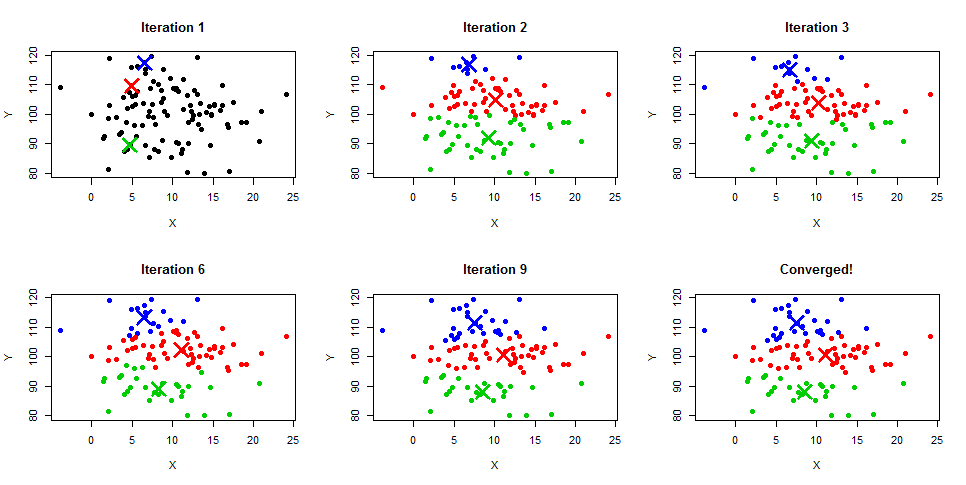
\includegraphics[width = 0.5\textwidth]{img/cluster/kmeans.png}
      \caption{Esempio di funzionamento dell'algoritmo $k-$means.}
      \label{img:k-means}
\end{figure}
Questo algoritmo è molto semplice da implementare e richiede un tempo di calcolo
pari a: $\mathcal{O}(t \cdot k \cdot n)$ con:
\begin{itemize}
      \item $n$ cardinalità dell'insieme dei dati.
      \item $k$ numero di cluster.
      \item $t$ numero di iterazioni del ciclo (avendo quindi $kt << n$)
\end{itemize}
\textbf{k-means} ha diversi problemi:
\begin{itemize}
      \item Ha una sensibilità rispetto alla scelta dei centroidi iniziali,
            sperimentalmente si è dimostrato che brutti valori iniziali
            invalidano l'intero processo.
      \item Non si può predire il numero di cluster non conoscendo a priori i
            dati, in aggiunta, non esiste un $k$ ottimale e non ci sono proprietà
            che ce lo possano suggerire. Si possono però usare delle
            approssimazioni studiando gli iperparametri. Non sapendo a priori il
            numero di $k$ posso ottenere scarsi risultati magari non avendo
            abbastanza centroidi. Adattarsi ad un numero “errato” di centroidi
            può portare a risultati “sporchi”.
      \item L'algoritmo è sensibile rispetto alle dimensioni geometriche che
            hanno le istanze nello spazio, infatti, lavorando sui centroidi
            potrebbe classificare in modo errato questo dettaglio, non
            distinguendo i corretti insiemi di punti.
      \item L'algoritmo è sensibile anche alla densità degli esempi, infatti se
            non avessimo $k$ sufficientemente grande allora si potrebbe arrivare
            a classificazioni errate.
\end{itemize}
In ogni caso, questo algoritmo mappa sensatamente i vari elementi in base alle
loro caratteristiche e quindi è un approccio parecchio usato, essendo generalmente
efficacie. Per risolvere i problemi introdotti precedentemente, si può provare
ad aumentare il numero di cluster, unendo poi, in un secondo passaggio, i vari
cluster secondo certi criteri, magari avendo una netta separazione lineare tra
cluster. Così si possono risolvere i problemi legati alla distribuzione geometrica
degli esempi, però rimane sempre il problema dell'identificare le posizioni di
inizializzazione dei centroidi migliori.
\section{Silhouette}
Per misurare le prestazioni di clustering bisogna capire come classificare i
risultati. Si usa la misura di \textbf{silhouette} per capire se un clustering è
migliore di un altro. Tale misura si basa sempre sul concetto di distanza.

Fissando una misura di distanza tra istanze $i, j$ ($d(i, j)$), definiremo:
\begin{enumerate}
      \item Distanza media \textbf{intra-cluster}, ovvero simiglianza tra
            elementi dello stesso cluster. Per ogni elemento $i$ di un cluster
            $C_I$, si calcola:
            \begin{equation}
                  a(i) = \frac{1}{|C_I| - 1} \sum_{j \in C_I, j \neq i} d(i, j)
            \end{equation}
            si divide per $|C_I| - 1 $ perché non si considera la distanza tra
            un elemento e se stesso.
      \item Distanza media \textbf{inter-cluster}, ovvero simiglianza tra un
            elemento di un cluster rispetto a tutti gli elementi tra gli altri
            cluster.  Per ogni elemento $i$ di un cluster $C_I$, si calcola:
            \begin{equation}
                  b(i) = \min_{K \neq I} \frac{1}{|C_K|} \sum_{j \in C_K} d(i, j)
            \end{equation}
            si divide per $|C_K|$ perché si considera la distanza tra un elemento
            e tutti gli elementi di un altro cluster.

            Si prende il minimo per confrontarlo con il cluster più vicino, anche
            detto \textbf{neighbor cluster}.
\end{enumerate}
ottenendo quindi la silhouette per il punto i come:
\begin{equation}
      s(i) = \frac{b(i) - a(i)}{\max\{a(i), b(i)\}}
\end{equation}
La qualità viene quindi visualizzata da un diagramma \ref{fig:silhouette} che
studia la silhouette al variare di $k$ per ogni valore di ogni attributo
(mettendo per ogni attributo in alto i valori più studiabili).
\begin{figure}
      \centering
      \begin{subfigure}[b]{0.6\textwidth}
            \centering
            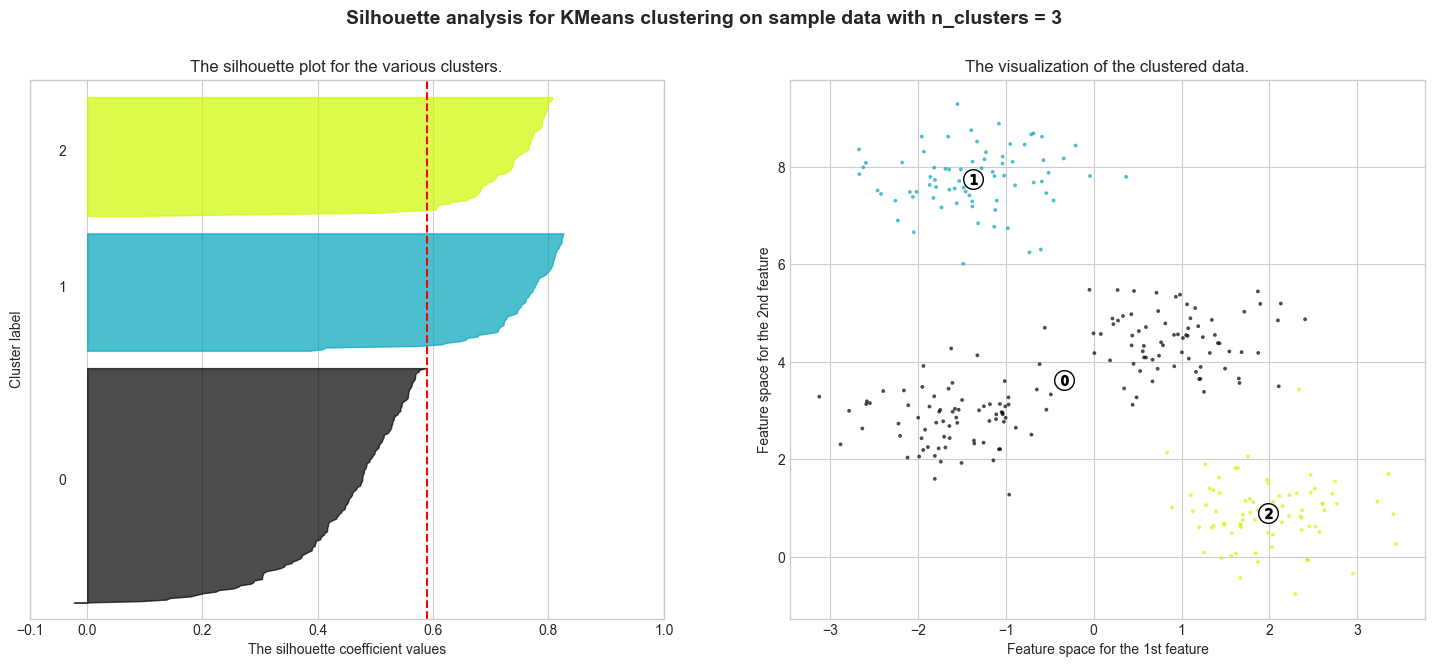
\includegraphics[width=\textwidth]{img/cluster/silhouette1.png}
            \caption{}
            \label{fig:silhouette1}
      \end{subfigure}
      \hfill
      \begin{subfigure}[b]{0.6\textwidth}
            \centering
            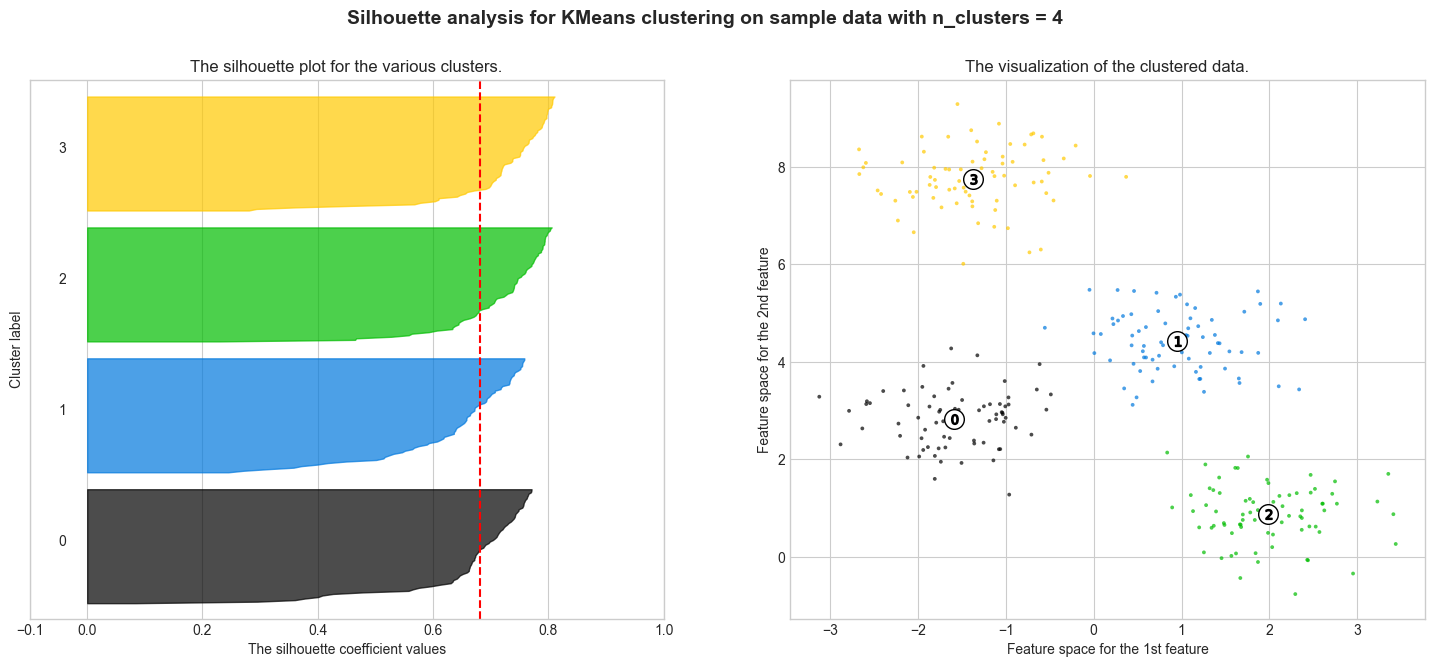
\includegraphics[width=\textwidth]{img/cluster/silhouette2.png}
            \caption{}
            \label{fig:silhouette2}
      \end{subfigure}
      \caption{Esempio di diagramma di silhouette.}
      \label{fig:silhouette}
\end{figure}
La media $s(i)$ su tutti i punti di un cluster è una misura di quanto siano
strettamente raggruppati tutti i punti del cluster. Pertanto, la media $s(i)$ su
tutti i dati dell'intero set di dati è una misura di quanto adeguatamente i dati
sono stati raggruppati. Se ci sono troppi o troppo pochi cluster, come può
accadere quando una scelta sbagliata di $k$ viene utilizzata nell'algoritmo di
clustering, alcuni dei cluster mostreranno tipicamente linee molto più strette
rispetto al resto nel diagramma di silhouette. Quindi grafici e media di
silhouette possono essere utilizzati per determinare il numero “naturale” di
cluster all'interno di un set di dati.

Il valore della silhouette può variare da $-1$ a $1$, dove un valore alto indica
che gli oggetti sono ben raggruppati nel cluster e lontani dai cluster vicini.
Se molti punti hanno un valore alto, allora la configurazione del cluster è
appropriata. Se molti punti hanno un valore basso o negativo, allora la
configurazione del cluster può avere troppi o troppo pochi cluster.
Ad esempio:
\begin{itemize}
      \item Un valore medio della silhouette maggiore di $0,7$ è considerato un
            raggruppamento solido.
      \item Un valore medio della silhouette inferiore a $0,2$ indica che i
            dati potrebbero essere stati raggruppati in cluster errati.
\end{itemize}
La silhouette è utile quando i cluster hanno forme arbitrarie, e potrebbe avere
problemi se i cluster hanno forme irregolari. Posso usare qualunque misura di
distanza.
\chapter{Performance Evaluation}
In machine learning una delle fasi più importanti è la valutazione del modello,
utile per capire la sua bontà e per avere delle metodologie di confronto con gli
altri.

Innanzitutto per valutare il modello non si considerano gli errori, calcolati come
scarto, delle predizioni sui dati di training. Questo perché successivamente si 
otterranno nuovi dati completamente differenti da quelli utilizzati per la fase
di training, invalidando la metrica calcolata.

La valutazione del modello permette fin da subito di rilevare eventuali comportamenti
di underfitting o di overfitting. Queste dinamiche vengono illustrate nella figura 
\ref{fig:overfitting-vs-underfitting}, in cui si può notare che un modello all'aumentare
della sua complessità si avrà tre fasi:
\begin{itemize}
    \item \textbf{fase di underfitting}: fase in cui il modello è ancora semplice
    per cui gli errori sul training e sul test sono elevati. Questo significa che
    si è in underfitting perché il modello non fitta bene sul training e, in aggiunta,
    non riesce a generalizzare.
    \item \textbf{fase ideale}: fase in cui il modello ha una complessità adeguata
    per cui non è troppo semplice da andare in underfitting e non è troppo complesso
    da andare in overfitting. Questa fase è ideale perché si ha un buon fit sul training
    e una buona generalizzazione sul test set
    \item \textbf{fase di overfitting}: fase in cui il modello è troppo complesso
    quindi si fitta molto bene sul training ma non riesce a generalizzare sul test.
    Questo comporta errori molto piccoli sul training, con un conseguente aumento
    degli errori sul test.
\end{itemize}

\begin{figure}[!ht]
    \centering
    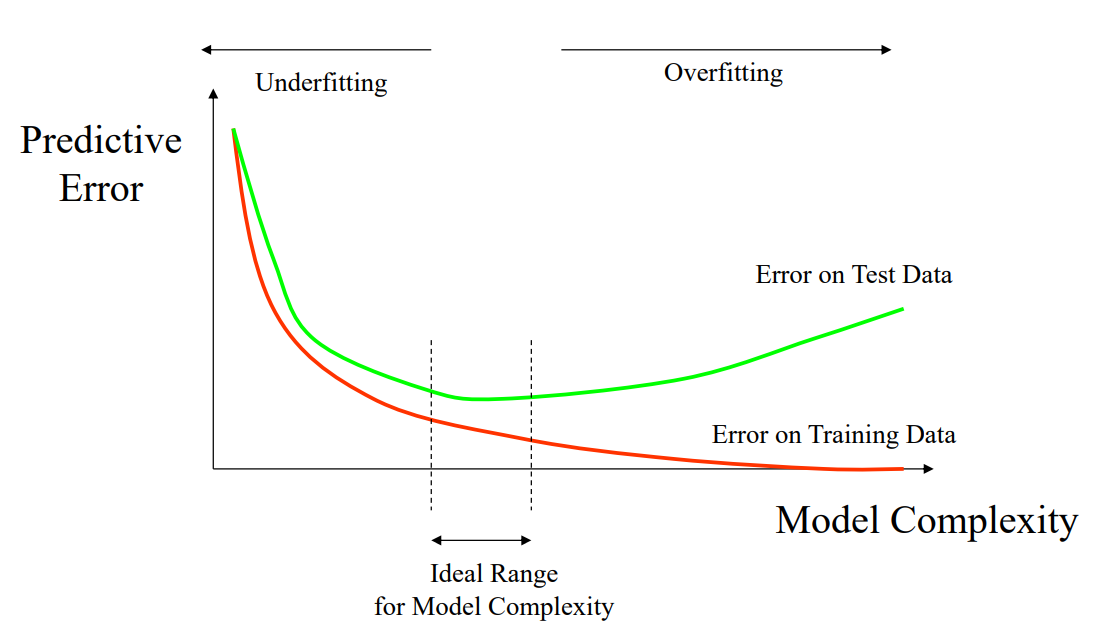
\includegraphics[width=0.7\textwidth]{img/performance evaluation/overfitting_vs_underfitting.png}
    \caption{Rappresentazione dell'overfitting e underfitting}
    \label{fig:overfitting-vs-underfitting}
\end{figure}

Le metriche di valutazione evidenziano tre componenti:
\begin{itemize}
    \item bontà del modello sul train
    \item bontà del modello sul test
    \item complessità del modello (quanti parametri): spazio, tempo in termini di $O$
\end{itemize}

Per le metriche sarà fondamentale introdurre la \textbf{matrice di confusione}, in cui 
\begin{equation}
    T[i,j] = \# \ \text{degli esempi etichettati come} \ i \ \text{predetti come classe} \ j
\end{equation}
Se si è nel caso di classificazione binaria allora:
\begin{itemize}
    \item $i=0, j=0$, true positive, \textbf{TP}: esempi positivi predetti come positivi
    \item $i=0, j=1$, false negative, \textbf{FN}: esempi positivi predetti come negativi
    \item $j=1, j=0$, false positive, \textbf{FP}: esempi negativi predetti come positivi
    \item $j=1, j=1$, true negative, \textbf{TN}: esempi negativi predetti come negativi 
\end{itemize}
L'obiettivo sarà quello di massimizzare la diagonale e minimizzare il resto.
\section{Metriche di valutazione}
Le metriche di valutazione sono differenti e si possono calcolare in modo aggregato
su tutte le classi oppure si possono calcolare su una classe alla volta e in un 
secondo momento aggregarle secondo delle medie.

Le metriche aggregate sono:
\begin{itemize}
    \item \textbf{Tasso di errore}:
    Metrica più naturale che consiste nel calcolo della proporzione degli errori su 
    tutto l'insieme di istanze dato in input al modello. Gli errori possono essere 
    calcolati secondo lo scarto o secondo le distanze.
    \item \textbf{Accuracy}:
    Misura la proporzione di istanze correttamente classificate su tutto l'insieme
    dato in input sul set.
    \begin{equation}
        Ac = \frac{TP+TN}{TP+TN+FP+FN}
    \end{equation}
    \item \textbf{Precision}:
    La precision misura la proporzione di esempi positivi predetti come positivi (TP)
    sul numero totale di esempi predetti come positivi.
    \begin{equation}
        P=\frac{TP}{TP+FP}
    \end{equation}
    \item \textbf{Recall}:
    La recal misura la proporzione di esempi positivi predetti come positivi (TP) sul
    numero totale di esempi positivi predetti come positivi ed esempi positivi predetti
    come negativi.
    \begin{equation}
        R=\frac{TP}{TP+FN}
    \end{equation}
    \item \textbf{F-measure}:
    La F-measure calcola la media armonica della precision e della recall.
    \begin{equation}
        \frac{2\cdot P\cdot R}{P+R}
    \end{equation}
\end{itemize}

Le ultime tre le calcoleremo sulle singole classi:
\begin{itemize}
    \item 
\end{itemize}


Queste misurare non le useremo sulle classi aggregate ma sulle singole classi
Se 3 classi allora abbiamo 3 misure di precision, recall, f-measure


PEr aggregare queste misurare useremo:
\begin{itemize}
    \item macro avg: fa la media tra le diverse classi delle singole metriche 
    (classi con uguale importanza)
    \item micro avg: media pesata della performance rispetto alla cardianlità 
    della classe (classe con diversa importanza) (possiamo specificare un peso 
    a piacere l'importante che si garantisca il range della metrica)
\end{itemize}


Per confrontare i modelli si utilzizano le curve ROC e mettono a confronto TP rate
e FP rate. La curva ROC non sono altro che la valutazione del modello con diverse
soglie decisionali del modello da 0 a 1, EX: Bayes si sceglie al posto di 0.5 a 0.8 
Più la soglia tende a 1 allora si ha un modello conservativo miglioreremo la precision
peggiorando la recall
Più abbassiamo la soglia si aumenta la recall ma si abbassa la precision.
La ROC si costruisce eseguendo i modelli con treshold diverse e si ricalcola la 
matrice di confusione diversa e quindi TPR e FPR differenti.

Nel confronto tra modelli avremo una curva per ogni modello e questo permette di 
studiare il suo comportamento. Generalmente si confronta il singolo modello con il
classificatore perfetto (verde) e quello randomico (rosso). Il modello migliore è
il dominante. Quando le linee si intersecano allora si deve studiare l'area sottesa 
all'area AUC (scalare). Quindi prendo quello con AUC maggiore. Può essere utilizzato 
in trainig e testing.
Hanno delle limitazioni:
- AUC sono inutili quando le classi hanno diversa importanza 
- sensibile allo sbilanciamento perché una classe sarà più pesante sui risultati


Curve di apprendimento sono delle curve che possiamo disegnare che dicono al variare
della numerosità del campione come si comporta il modello in termini di accuratezza.
Le barre blu rappresentano la varianza della predizione. I punti rappresentano
le media della metrica scelta delle singole esecuzioni del metodo eseguiti su tutte le combinazioni
di 5 cambino di training. 
Quanti dati sono necessari per avere un modello con performance accettabile in termini
di tempo di apprendimento e della performance. Molto pesante ma spesso si costruisce 
parzialmente.

Prob grande => 10000 istanze 
Più grande il campione allora si effettuerà una suddivisione train test 80 20

Se il modello deve essere messo in produzione allora effettuo il training su tutto 
dataset.

I dati di test non devono essere usati per il tuning degli iperparametri. GLi
iperparametri possono essere i k cluster o anche le soglie del modello e si trovano
sul validation.

Per dataset piccoli si esegue train test più volte in crossvalidation.

Per la generazione degli insiemi per crossvalidation spesso chiedono la stratificazione
ovvero se ho una classe popolosa allora questa deve essere uguale sia in training sia in
test. Si deve sempre stratificare (generalmente si usa k=10 fold). 

Quando abbiamo dataset estremamente piccoli <100 istanze e quindi si usa la tecninca
di leave-one-out. Crossvalidation di 1 test e tutto il resto training

\section{Affidabilità delle misure di performance}
Ogni iterazione della k-fold mi da una misura di performance, posso calcolare la media
tra tutte le performance. Non si può utilizzare la media per confrontare perché 
perdiamo la variabilità. Quello che si fa è stimare gli intervalli di confidenza
perché:
\begin{itemize}
    \item si capisce la posizione della media
    \item ci da la robustezza  (ampiezza intervallo di confidenza) meglio quello
\end{itemize}
2 modelli

stessa media , il primo IC 0.7,0.8 mentre il secondo 0.5 e 1, il migliore è quello
col più piccolo intervallo. Se gli intervalli non si sovrappongono e hanno la 
stessa ampiezza è la situazione migliore.

Altro approccio di confronto tra modelli si usa il test di significatività 
- test paired quando entrambi i modelli hanno imparato nello stesso modo sugli stessi dati
- test unpaird altrimenti

Non guardare solo la performance numerica
Considera sempre la complessità
\chapter{Deep Learning}
Le principali tipologie di apprendimento sono:
\begin{itemize}
      \item \textbf{Supervisionato} (Supervised): i dati utilizzati per
            l'apprendimento sono etichettati (label).
      \item \textbf{Non supervisionato} (Unsupervised): i dati utilizzati per
            l'apprendimento non sono etichettati.
\end{itemize}
Inizialmente, le architetture di deep learning sono state composte da
particolari strutture simili agli enconder-decoder chiamate \textbf{autoencoder}
(figura \ref{fig:autoencoder}). Queste strutture sono reti neurali, costruite
con una particolare struttura a clessidra, il cui compito è quello di imparare
come ricostruire l'input.
\begin{figure}[!ht]
      \centering
      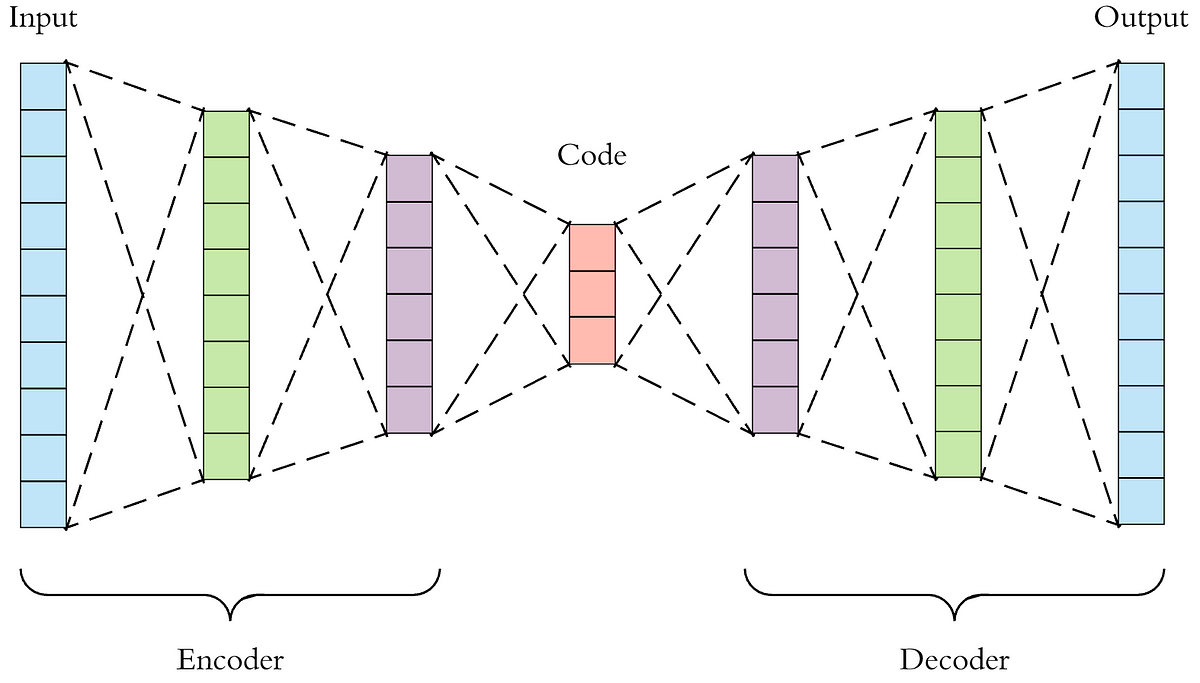
\includegraphics[width=0.5\textwidth]{img/reti/autoencoder.png}
      \caption{Autoencoder}
      \label{fig:autoencoder}
\end{figure}
La metodologia di apprendimento utilizzata dagli autoencoder è unsupervised.
Nella realtà non è del tutto non supervisionata in quanto si ha un \textbf{fake
      task}, ovvero si adotta una metodologia supervisionata in cui non si ha
una label da predire, ma si vuole ottenere l'input stesso. L'obiettivo di
queste reti è quindi quello di ridurre l'errore sulla ricostruzione dell'input.

Il loro risultato è dovuto alla loro struttura, in particolare risulta utile la
codifica ottenuta nel collo di bottiglia che separa la rete in due:
\begin{itemize}
      \item \textbf{Enconder}: impara a codificare l'input utilizzando poche
            informazioni (funzione di codifica, spesso segnata come $Enc(X) = Z$).
      \item \textbf{Deconder}: impara a decodificare l'input partendo da poche
            informazioni (funzione di decodifica, spesso segnata come $Dec(Z) = Y$).
\end{itemize}
L'algoritmo di apprendimento di queste reti spesso è una delle tante
implementazioni di backpropagation, applicandolo su ciascun neurone di uscita.
Più precisamente l'apprendimento si effettua definendo una \textbf{funzione di
      loss} $\mathcal{L}$ che calcolerà la distanza tra l'output del decoder $Y$
e l'input $X$ della rete:
\begin{equation}
      \mathcal{L} = \| X - Y \|
\end{equation}
Per gli autoencoder si deve obbligatoriamente avere sempre una struttura a
clessidra con la strozzatura centrale, la quale permette di generare la codifica
e separare le due reti. In aggiunta, l'architettura non prevede che ci siano
collegamenti tra encoder e decoder altrimenti la codifica nella strozzatura non
sarebbe più consistente.

L'encoder della rete non fa altro che trovare una codifica dell'input in uno
spazio di dimensioni ridotto, questo significa che equivale a calcolare la PCA
sull'input, con la differenza che uno utilizza una rete neurale mentre l'altro
è un processo iterativo basato sugli autovalori e autovettori. Più precisamente
PCA cambia il sistema di riferimento dello spazio in modo tale che gli assi
siano in direzione della massima variabilità. Vista questa dualità con la PCA,
gli autoencoder possono trovare una rappresentazione dell'input a dimensioni
minori per risolvere dei task specifici. La rappresentazione codificata prenderà
il nome di \textbf{rappresentazione latente}.

L'autoencoder può essere utilizzato anche per effettuare task di classificazione
più precisamente si allena l'autoencoder e nel mentre si allena una rete che
prende la rappresentazione latente e la classifica. Quindi la rete sarà formata
da:
\begin{itemize}
      \item Encoder: $Z = Enc_{\theta_1}(X)$
      \item Classificatore: $\hat{y} = F(Z)$
      \item Decoder: $Y = Dec_{\theta_2}(Z)$
\end{itemize}
La loss dovrà essere l'unione delle loss del classificatore e dell'autoencoder.
\begin{equation}
      \mathcal{L} = \| X - Y \| + \| y - \hat{y} \|
\end{equation}

Le architetture odierne di deep learning si basano su strutture neurali e
utilizzano i \textbf{transformer} (figura \ref{fig:transformer}), componenti
neurali che prendono in input sia il nuovo input, sia un vecchio output del
transformer shiftato a destra. Sono componenti fondamentali per la generazione
di informazioni. L'apprendimento di queste reti si basa su strutture \textbf{feed
      -forward} e su componenti \textbf{Attention}, quest'ultimi fondamentali
perché permettono l'effettivo cambiamento dei valori.
\begin{figure}[!ht]
      \centering
      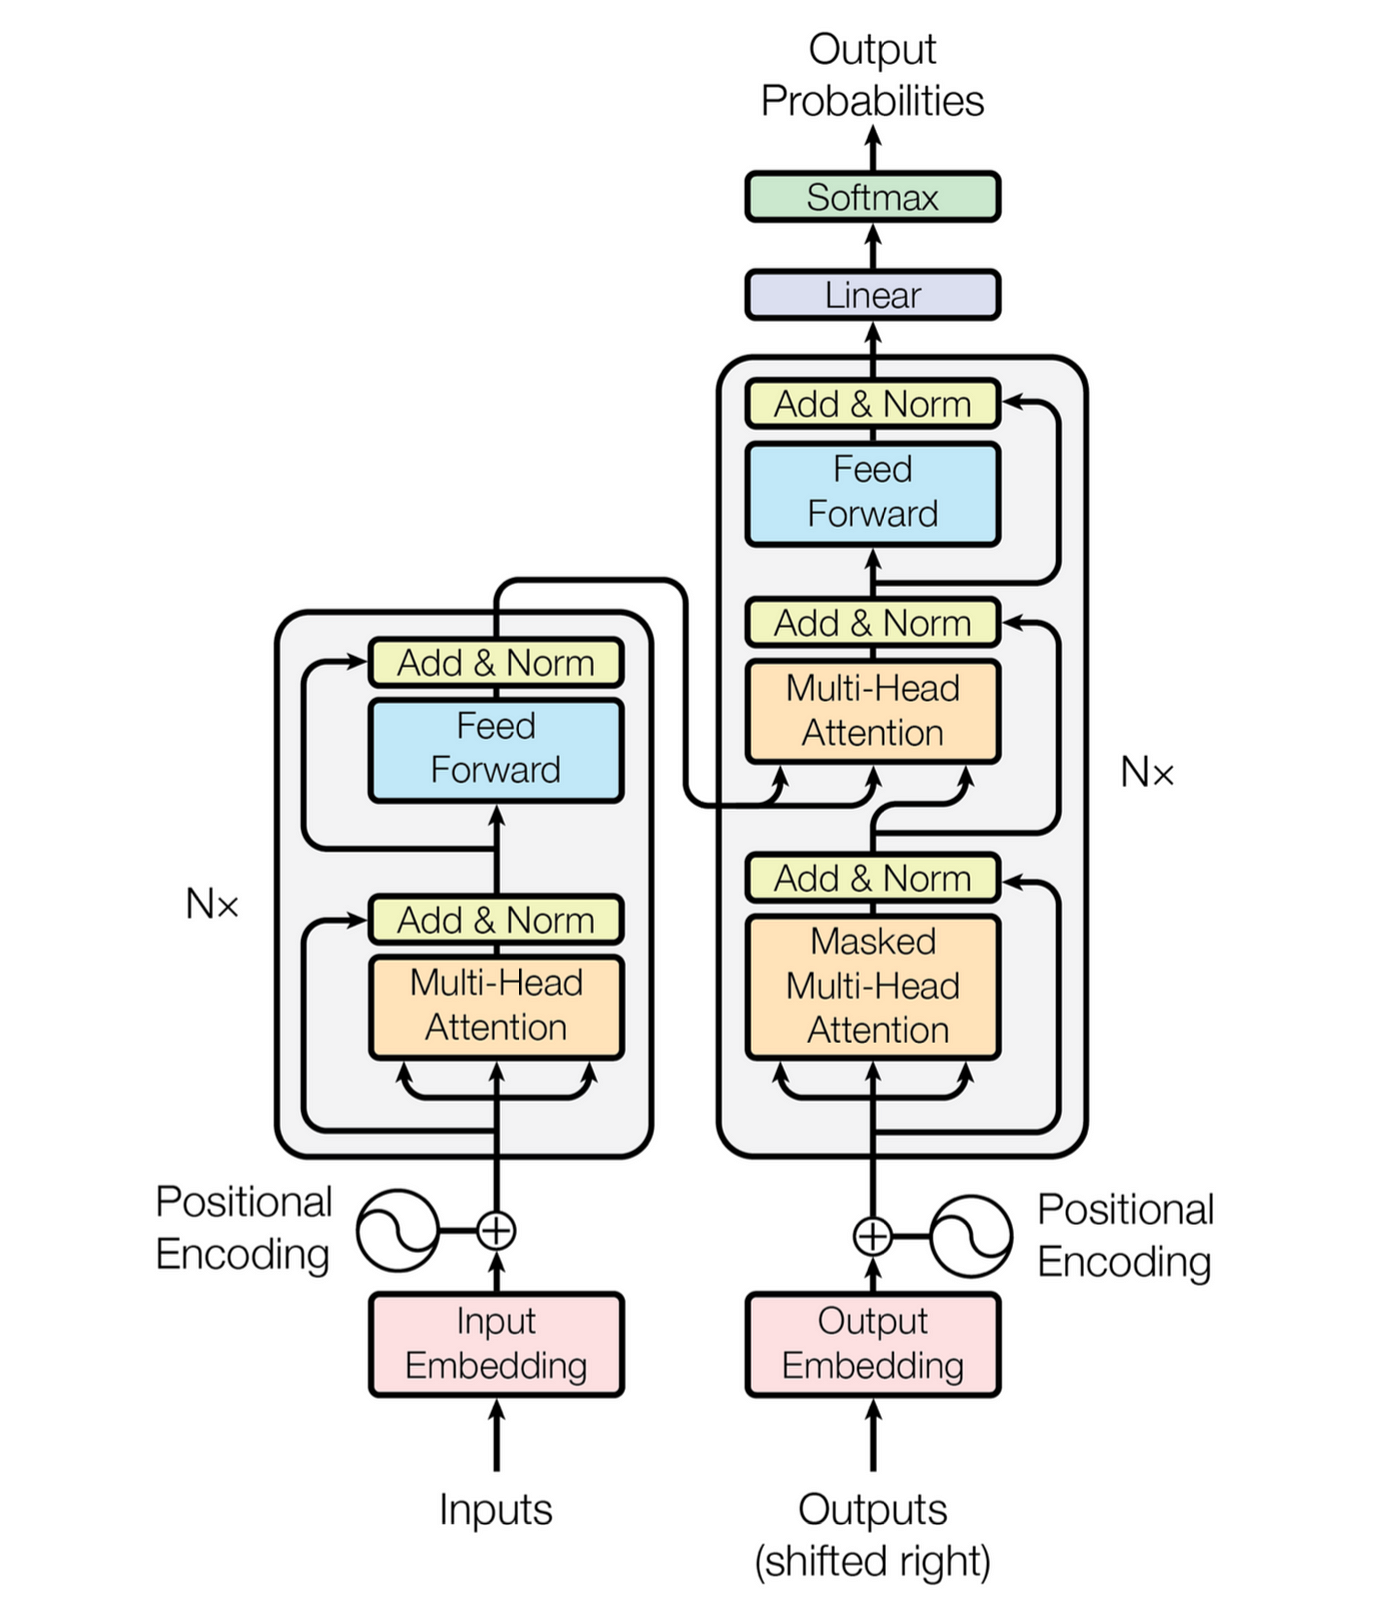
\includegraphics[width=0.5\textwidth]{img/deepl/transformer.png}
      \caption{Struttura di un transformer}
      \label{fig:transformer}
\end{figure}
Prima di arrivare ai transformer si è passati dagli autoencoder, a
\textbf{Word2Vec}, un modello neurale utilizzato per problemi di \textbf{NPL}.
Più precisamente si occupa di associare per ogni parola del linguaggio un vettore
di numeri reali, in questo modo è possibile rappresentare le singole parole in
uno spazio $n$-dimensionale. Questa proprietà ha permesso di scoprire una
proprietà: parole simili vengono rappresentate in una regione vicina dello
spazio. Questo è dato dal fatto che le reti vengono allenate su tutti i testi
raggiungibili e l'assegnamento del vettore si effettua in base a quante volte
due parole vengono veste vicine in una frase. Quindi la rete riesce a codificare
come vettori simili parole simili, infatti c'è una corrispondenza geometrica col
significato.

Successivamente si è passati ai \textbf{denoising autoencoder} (figura
\ref{fig:denoising}), ovvero rimozione del rumore e ricostruzione dell'input
originale. Queste reti vengono allenate dando in input il dato sporcato in
precedenza, successivamente l'output viene confrontato con l'input originale.
\begin{figure}[!ht]
      \centering
      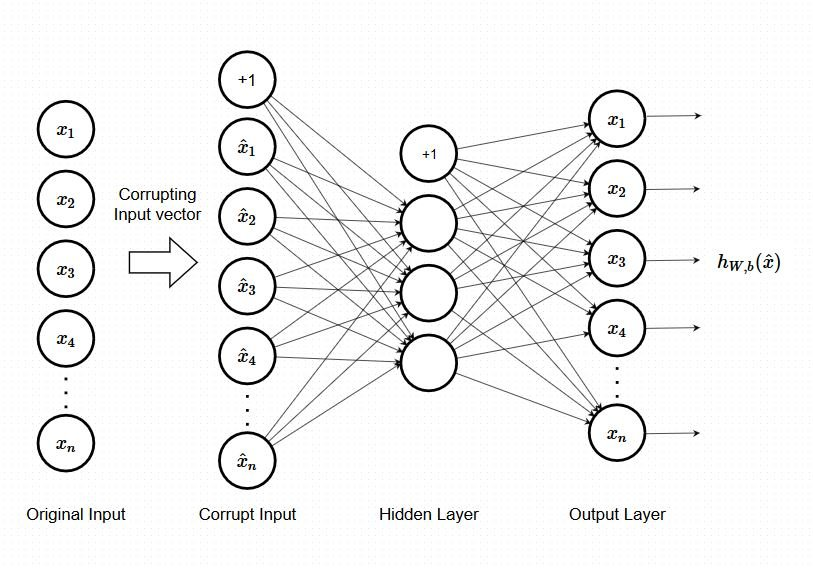
\includegraphics[width=0.5\textwidth]{img/deepl/DenoisingAutoencoder.png}
      \caption{Denoising autoencoder}
      \label{fig:denoising}
\end{figure}
Questa tipologia di rete è nata con lo scopo di impedire all'autoencoder di
imparare la funzione identità, questo perché quando l'autoencoder ha dimensioni
troppo elevate, la rete impara a copiare l'input in output senza effettuare
nessuna trasformazione. Per questo motivo si è deciso di aggiungere del rumore
all'input, in modo da rendere più difficile la ricostruzione dell'input
originale.

In seguito, sono stati introdotti i componenti \textbf{Attention} (figura
\ref{fig:attention}), composti da 3 elementi in input e il suo compito è di
assegnare in automatico diversi pesi agli elementi in input. Queste reti
permettono quindi di cambiare i pesi degli input portando a dei vantaggi notevoli,
per esempio, si possono interpretare parole ambigue in base al contesto.
\begin{figure}[!ht]
      \centering
      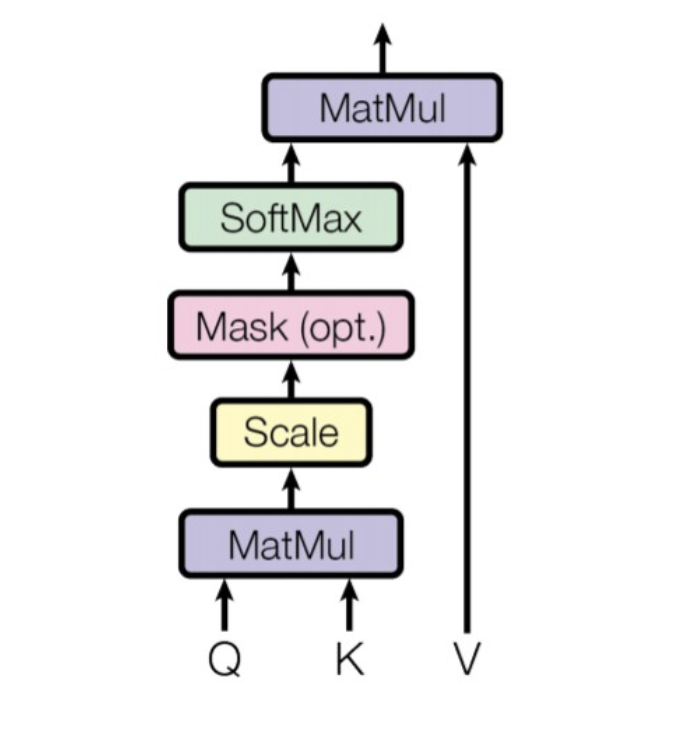
\includegraphics[width=0.5\textwidth]{img/deepl/attention.png}
      \caption{Componente Attention}
      \label{fig:attention}
\end{figure}
Infine, si è passati ai transformer, un modello che evita la ricorrenza e si
basa invece interamente sui meccanismi di attention per valutare le dipendenze
dei dati tra input e output. Utilizzando strutture encoder-decoder, rimuovendo
la ricorrenza in favore dei meccanismi di attention.
%% FONTE: https://paperswithcode.com/method/transformer

I modelli di deep learning vengono allenati in 2 fasi:
\begin{itemize}
      \item \textbf{pre-training generico}: allenamento non supervisionato, si
            allena la rete in modo generale senza specificare un particolare
            task. Questa fase è la più pesante e permette di definire un primo
            stato di partenza dei parametri.
      \item \textbf{fine tuning}: si prende la rete pre-allenata e si addestra
            per un task specifico utilizzando la metodologia supervisionata.
\end{itemize}
In questo modo è possibile ridurre i tempi di addestramento e rendere
riutilizzabile la stessa rete per task simili.

Alla fine si arriva alla creazione di reti più complesse come GPT, basata sempre
su transformer e attention, ma addestrata in 2 fasi, con la possibilità di
effettuare del reinforcement learning per migliorare ancora di più i risultati.

\chapter{Ripasso di algebra lineare}
Per praticità ripasseremo i concetti fondamentali facendo riferimento a $\mathbb{R}^2$,
formato quindi da elementi, dette coordinate, che sono coppie ordinate $(x_1,x_2)$
(rappresentabili con un punto nel piano o con un segmento orientato con partenza
nell'origine e destinazione nelle coordinate del punto nel piano).

Ricordiamo le operazioni fondamentali, dati $R$ pari a $(x_1,x_2)$ e $Q$ pari a $(x_3,x_4)$
\begin{itemize}
    \item addizione: $P+Q=(x_1+x_3, x_2+x_4)$
    \item prodotto per uno scalare $\lambda\in\mathbb{R}$: $\lambda\cdot R=(\lambda\cdot x_1,\lambda\cdot x_2)$
    \item prodotto scalare tra vettori: $\langle P,Q\rangle\equiv P\cdot Q^T = \sum_{i=1}^n r_i\cdot q_i$
          (dove $r_i$ e $q_i$ sono rispettivamente gli elementi di $R$ e $Q$ all'indice $i$)
\end{itemize}

Ricordiamo la \textit{norma} di un vettore $X$:
\begin{equation}
    \lVert X \rVert=\equiv\sqrt{X\cdot X^T}=\sqrt{\sum_{i=1}^n x_i\cdot x_i}=\sqrt{\langle X,X\rangle}
\end{equation}

Con $X=0$ indichiamo il \textit{vettore nullo} (che ha anche norma nulla).

Definiamo il \textit{versore} (\textit{vettore unitario}) come:
\begin{equation}
    \frac{X}{\lVert X \rVert},\ \ \ X \neq 0
\end{equation}
In $\mathbb{R}^2$ l'angolo $\theta$ sotteso tra due vettori $X$ e $Y$ è:
\begin{equation}
    \cos\theta=\frac{\langle X,Y\rangle}{\lVert X \rVert\cdot \lVert Y \rVert}
\end{equation}

La proiezione di un vettore $X$ sul vettore $Y$ è:
\begin{equation}
    X_Y = \lVert X \rVert \cdot \cos\theta
\end{equation}
Si hanno quindi tre casi:
\begin{enumerate}
    \item $\theta < 90 \iff \langle X,Y\rangle >0$
    \item $\theta > 90 \iff \langle X,Y\rangle <0$
    \item $\theta = 90 \iff \langle X,Y\rangle =0$
\end{enumerate}
(quindi disegnando una retta sul piano tutti i punti sopra di essa apparterranno
ad una certa classe e quelli sotto ad un'altra).

Posso definire una retta $r$ che passa per l'origine in  $\mathbb{R}^2$ assegnando
un vettore $W=(w_1,w_2)$ ad essa ortogonale, infatti tutti i punti, ovvero
vettori, $X=(x_1,x_2)$ sulla retta sono ortogonali a $W$:
\begin{equation}
    \langle W,X\rangle=w_1\cdot x_1+w_2\cdot x_2=0
\end{equation}


Quindi la retta (ovvero l'iperpiano) mi separa due semispazi, a seconda che
$\langle X,W\rangle$ sia strettamente positivo o strettamente negativo.

Generalizzando ora a $n$ dimensioni ho che, dato l'iperpiano $h$ (di dimensione $n-1$):
\begin{itemize}
    \item se $h$ passa dall'origine allora si ha l'equazione $\langle X,Y\rangle=0$
    \item se non passa per l'origine $\langle X,Y\rangle +b=0$
\end{itemize}

I vettori in un iperpiano si proiettano tutti nello stesso modo e i punti ad un
lato e all'altro dell'iperpiano sono distinti dal fatto che $\langle X,Y\rangle +b$
sia strettamente positiva o strettamente negativa.
\end{document}